
\documentclass[english]{isasthesis}

\usepackage[utf8]{inputenc}
\usepackage{wrapfig}
\usepackage{graphicx}
\usepackage{amsmath}
\usepackage[numbers]{natbib}
\usepackage{multirow}


%%%%%%%%%%%%%%%%%%%%%%%%%%%%%%%%%%
% Edit notation.tex if necessary
%%%%%%%%%%%%%%%%%%%%%%%%%%%%%%%%%%

%%%%%%%%%%%%%%%%%%%%%%%%
% Document properties
%%%%%%%%%%%%%%%%%%%%%%%%

\title{Magnetic Sensor Characterization and Signal Conditioning\\ for Position and Speed Estimation\\ of BLDC Motors}
\author{Julien Aziz}
\date{07. September 2020}

\thesistype{Bachelor Thesis}
\firstsupervisor{Dipl.-Phys. Jana Mayer}
\secondsupervisor{M.Sc. Ajit Basarur}

%%%%%%%%%%%%%%%%%%%%%%%%
% Document
%%%%%%%%%%%%%%%%%%%%%%%%

\begin{document}
    \maketitle
    \begin{abstract}
        BLDC Motors are widely used technologies in several areas due to their advantageous size, cost and good controllability. When controlling such motors, the availability and precision of motor state information are urgently required. Previous works identified a dependency between the observable magnetic flux and the rotor position. Based on this correlation, a new feedback technique was developed, estimating the rotor's position and the speed simultaneously. While the estimation showed good results, the setup suffers from unnecessary complexity caused by the used sensor and unfavourable implementation decisions. \\ \\
In this thesis we condition the observations provided by the sensor and investigate the roots of two unexpected signal conditions. Namely, an observable distortion in the signal shape and an undesired speed dependency. In order to perform an elaborate sensor characterization, a new data preparation technique is presented. Furthermore, the spatial sensor arrangement will be evaluated to gain additional information about the measurement behaviour. Based on the obtained characteristics, alternative measurement positions are considered to avoid undesired magnetic influences. Subsequently, various approaches of System Identification are applied to construct a "deconvoluting" system, that eliminates the undesired speed dependency. Based on this system and the probed sensor positions, a new low-complex measurement model is developed. This technique is capable of estimating the system states with a one dimensional measurement variable and a simple sinusoidal term.  
    \end{abstract}
    \maketoc
    
    \chapter{Introduction}\label{introduction}
    Various technologies rely on precisely controlled electrical motors. In modern scientific areas such as automation technology and robotics, efficient measurement techniques are required in order to automatically perform precise transpositions. The crucial feedback includes information about the current state of the driving motor. This knowledge have to be provided at any given time. In case of BLDC Motors, precise motor operations are performed with the Field-Oriented Control
(FOC) algorithm which requires an accurate feedback of the rotor's position and rotational speed \cite{lee2009comparison}. Such motors produce a measurable magnetic flux during the regular operation due to the rotating permanent magnets. \\ \\
    In \cite{fabian} a new motor feedback-system was developed where the valuable motor states are estimated by observing the magnetic flux density at the backside of the motor. While the estimation approach showed precise results and was further improved in \cite{mariana}, the implementation suffers from an ill-conditioned measurement signal. More precisely, the integrity of the obtained magnetic field values is not as pure as expected but corrupted by some undesired influences. Additionally, we observe a speed dependent signal transformation with low-pass filter characteristics. These disturbances significantly increase the difficulty of implementing alternative estimation techniques. Consequently, the estimation algorithms themselves involve a substantial complexity. Beside some prior assumptions about the undesired influences, detailed knowledge about the source of these disturbances is not available.\\\\
    In this thesis, we investigate the unexpected signal conditions in order to obtain a detailed characteristic of the disturbances. This investigation includes an elaborate evaluation of the sensor position within the measurement setup. Additionally, we provide a new data simulation technique, defining the base for an extensive analysis on the sensor output. To eliminate the undesired low-pass frequency response, we approach three different \textit{System Identification} techniques to obtain a "deconvoluting" system that reverts the disturbing behaviour. Furthermore, we decrease the dimension of the measurement variable, leading to a significant simplification of the overall estimation task. Based on the identified characteristics and the constructed "deconvoluting" system, we implement a new measurement model. This new technique provides precise estimation results but most importantly, involves a low complexity.\\ \\
    In Chapter \ref{theoretical background} we provide the fundamentals which are necessary to comprehend the identified characteristics. The following Chapter \ref{previous works} is dedicated to previous works, where we  present the established estimation model but also further discuss the unexpected signal conditions. Chapter \ref{sensor characterization} and \ref{signal conditioning} are the investigation parts of this work. We analyse the disturbing influences as well as identify appropriate methods to eliminate them. One of these considered methods is the following \textit{System Identification} approach in Chapter \ref{system identification}. Finally, in Chapter \ref{evaluation} we evaluate the identified approaches. A summary of this work is provided in Chapter \ref{fazit} with a further discussion about future work. 
    \chapter{Theoretical Background} \label{theoretical background}
The given background includes physical basics of the motor itself as well as a brief introduction for general state estimation. The presented state estimation is based on the theory of the popular Kalman Filter. Additionally, we discuss the basic procedure of System Identification. Further details about the specific implemented techniques will be described in the dedicated Chapter \ref{system identification}. 
    	\section{BLDC Motors}
    	 \begin{wrapfigure}{r}{0.5\textwidth}
                \begin{center}
                \includegraphics[width=0.4\textwidth]{figures/BLDC-Motor_1.jpg}
                \end{center}
                \caption{Overview of a typical BLDC Motor}
                \label{fig:bldc}
          \end{wrapfigure}
         Brushless DC (BLDC) electric motors are a variant of the widespread Permanent Magnet Synchronous Motors (PMSM). They are rapidly gaining popularity due to the various advantages over brushed DC motors such as better speed versus torque characteristics, low maintenance and high efficiency \cite{welekar2014development}. Regarding Figure \ref{fig:bldc}, the motor generally consists of two parts, namely a rotating piece in the middle and a fixed stator surrounding it. While the rotor commonly features 2-8 permanent magnets, the stator includes 6 coils, which are charged up during the regular motor operation. By energizing those coils, electromagnetic poles are induced which consequently attract/repel the permanent magnets on the rotor. The concept is to create a rotational magnetic field by polarizing the coils in a appropriate sequence so the rotor's magnets will constantly be attracted by the subsequent winding. Since such a procedure relies on information about the motor state, an accurate feedback on the rotor position and the rotation speed is required.\\ \\
    	\section{State Estimation}
    	 In case of BLDC Motors, the states must be known at any given time in order to produce a desired rotation. However, these properties in general are valuable information as they reflect the condition of the system. The approach of estimating these system states is required, when a direct measurement is too inaccurate, inefficient or simply not possible. A common technique is to observe an alternative measurable property and predict the desired system states by injecting an appropriate \textit{Estimator} with the observations. One of the most popular estimation approaches is the so called Kalman Filter, defining the base for the presented estimation task. 
			\subsection{Dynamic Systems} \label{dynamic systems}
			In order to derive the Kalman filter, a suitable mathematical definition for the system is required. Since in real-world sensor based systems the measurements can only be evaluated in certain time-points \(t = t_k \), the presented modelling will only concern discrete-time systems. To describe the dynamic system we use a state-determined model where its characteristic behaviour is defined by the response of a minimum set of variables \(\underline{x}_k\), denoted as the \textit{state vectors}. In terms of a mathematics description, those state vectors in combination with the initial states and the system inputs \(\underline{u}_k\), are sufficient to predict the future system states at any given time \cite{rowell2002state}. In practical applications, obviously the system noise has to be taken into account.\\ \\
			For the \textbf{linear} case, a discrete-time system can be described as given in \cite{simon2006optimal},
			\begin{align}\label{eq: LinSysEquation}
			\underline{x}_k &= \mathbf{A}_{k-1}\underline{x}_{k-1}+\mathbf{B}_{k-1}\underline{u}_{k-1}+\underline{\epsilon}_{k-1}, \\
			\underline{y}_k &= \mathbf{H}_{k}\underline{x}_{k}+\underline{v}_k.\label{eq: LinMeasEquation}
			\end{align}
			The so-called \textit{System Equation} \eqref{eq: LinSysEquation} includes the system matrix \(\mathbf{A}\) and the input matrix \(\mathbf{B}\) as well as the mentioned system state vector \(\underline{x}\), the input vector \(\underline{u}\) and the system noise \(\underline{\epsilon}\) of the previous time step. While the system properties \(\mathbf{A}\) and \(\mathbf{B}\) are determined by the system states, the output matrix $\mathbf{H}$ is defined by the condition of the measurement value $\underline{y}_k$. The measurement noise $\underline{v}$ as well as the system noise $\underline{\epsilon}$, represent the uncertainties of the system and are commonly assumed as zero-mean uncorrelated Gaussian noise. Thus, we define them as
			\begin{equation}
			\begin{aligned}\label{eq:noise}
					\underline{\epsilon}_{k-1} &\sim \mathcal{N}(\underline{0},\mathbf{Q}_{k-1}), \\
                    \underline{v}_{k} &\sim \mathcal{N}(\underline{0},\mathbf{R}_k).
			\end{aligned}
			\end{equation}
While we assumed linearity to this point, almost every real-world system contains non-linear components. We formulate those equations for the \textbf{non-linear} case as
\begin{align} \label{eq: NonLinSysEquation}
		\underline{x}_{k} &= f_{k-1}(\underline{x}_{k-1},\underline{u}_{k-1},\underline{\epsilon}_{k-1}), \\
        \underline{y}_{k} &= \underline{h}_k(\underline{x}_k, \underline{v}_k).\label{eq: NonLinMeasEquation}
\end{align}
	\subsection{Kalman Filter}
	\begin{figure}[t]
                \centering
                \includegraphics[width=1\textwidth]{figures/KF.jpg}
                \caption{Overview of the Kalman Filter estimation procedure}
                \label{fig:KF}
     \end{figure}
	The Kalman Filter (KF) is basically a recursive data processing algorithm, predicting the current system state by processing the available observations. The measurements represent a form of feedback and the predictions are accordingly adjusted  \cite{maybeck1982stochastic}. The fundamental concept of the KF can be separated into two essential parts, namely the \textit{Prediction} followed by the \textit{Update}. \\ \\
	In the Prediction an a priori estimation of the current state $\underline{x}_k^p$ is derived by applying the \textit{System Equation} \eqref{eq: LinSysEquation} on the previous estimation $\underline{x}_{k-1}^e$. The following Update represents the "feedback" of the KF, where the prior estimated state $\underline{x}_k^p$ is compared to the processed observation $\underline{y}_k$. Base for this comparison is the so called \textit{Measurement Function} \eqref{eq: LinMeasEquation}. The result is then processed to consequently adjust the  prior prediction. Thus, an optimal estimation $\underline{x}_k^e$ of the desired system states is obtained. This correction describes a weighting, defined by the so called \textit{Kalman Gain} $K_k$, derived through both system uncertainties \cite{mariana}. A schematic overview for the basic two-step structure of the KF can be seen in Figure \ref{fig:KF}. \\ \\
	The problematic of this estimation approach is the optimality of the estimation is restricted to linear systems with Gauss distributed noise. More precisely, the common KF technique requires a \textbf{linear} relationship between the system states $\underline{x}$ and the measured property $\underline{y}$. The estimation task in this work, involves in fact a \textbf{non-linear} relationship between the system states and the observe variable. Therefore, we utilise a modification of the common KF, namely the Extended Kalman Filter (EKF). \\ \\
	 The concept of this approximative filter is to estimate the states of a \textbf{non-linear} system by linearising the system equations around the previous estimation $\underline{x}_{k-1}^{e}$. Subsequently the typical KF procedure is applied to obtain the desired estimation. More about the linearisation step of the EKF as well as the general implementation details can be found in \cite{simon2006optimal}.
	 \section{System Identification}
	 A common problematic in the study of signal processing is the fact, that observable properties are often noise corrupted or emerge from a convolution with an unknown system. Hence, to comprehend the behaviour of such measured signals or to eliminate an undesired transformation, additional insight about the disturbing system is  necessary. The study of \textit{System Identification} addresses the challenge of precisely defining the complete dynamics of an unknown system by extracting the characteristics from available observations. The difficulty of this task is increased if only insignificant or none pre knowledge at all about the systems parameters is available. In such cases this task is termed \textit{black box} modelling \cite{sid}.\\ \\
	 The general concept of the System Identification is to firstly gather enough relevant data, which can be individually processed. After the dedicated observations are obtained, a suitable identification model is applied and subsequently validated. The number of available identification techniques is significant and even though the approaches vary widely in the specific approach, all feature the same basic idea. Namely, a structured investigation on the system response to a known excitation, represented by \textit{input}-\textit{output} observations. \\ \\
    	Consider an unknown linear system with a known input $u(k)$ and a measurable output $y(k)$ with respect to the time $k$. To define the relation between the in- and output one firstly has to assume a specific model structure that shall describe the unknown dynamics of the system. In case of linear systems, common structures are:
    	\begin{enumerate}
    		\item Differential Equation, where the relation is defined as
    		\begin{equation}\label{eq:differential}
    		y^{(n)}(k)+ a_1y^{(n-1)}(k)+\cdots+a_ny^{(0)}(k) = b_mu^{(n)}(k) + b_{m-1}u^{(m-1)}(k)+\cdots+b_0u^{(0)}(k). 
    		\end{equation}
    		\item Transfer Function Models, based on the Laplace transformed input-output signals, $\mathcal{L}\{u(k)\} = U(s)$ and $\mathcal{L}\{y(k)\} = Y(s)$ with the complex variable $s$. The relation is then defined by 
    		\begin{equation}
    		Y(s) = \frac{b_0s^m + b_1s^{m-1}+\cdots}{a_0s^m + a_1s^{n-1} + \cdots} U(s),
    		\end{equation}
    		or more commonly
    		\begin{equation}\label{eq:transfer function}
    		Y(s) = \frac{B(s)}{A(s)}U(s).
    		\end{equation}
    		\item Discrete State Space Models, defined as 
    		\begin{equation}\label{eq:state space}
    		\begin{aligned}
    		x_{k+1} &= \mathbf{A}x_k + \mathbf{B}u_k, \\
    		y_k &= \mathbf{C}x_k + \mathbf{D}u_k.
    		\end{aligned}   		    		
    		\end{equation}
    	\end{enumerate}
    	Hence, after the model structure was chosen, an appropriate identification technique is applied to obtain the unknown parameter vectors $\underline{a}$ and $\underline{b}$.\\\\
   The common procedure is to choose a set of suitable mathematical model structures and apply the individual identification techniques. The identified systems are then validated by exciting the model with input sets from independent measurements and comparing the according response to the real measurement outputs. If the model does not sufficiently reproduces the behaviour of the independent dataset, one has to consider an alternative identification or refine the datasets accordingly. In \cite{sid}, Lennart Ljung (2017) presented an overview of this common System Identification procedure which can be seen in Figure \ref{fig:sid loop}.\\ \\
	\begin{figure}[t]
    		\centering
    			\includegraphics[width=0.8\textwidth]{figures/identification_loop.jpg}   
    		\caption{The typical identification loop, presented in \cite{sid}}
    		\label{fig:sid loop}
    		\end{figure}
	\chapter{Previous Work}\label{previous works}
	In \cite{fabian} a new state estimation approach for BLDC Motors was developed. The idea emerged as common state of the art methods such as inbuilt Hall-sensors or optical encoders suffer under inaccuracy or cost-inefficiency. Additionally, most of the available sensor based feedback systems measure either the angular position or the rotation speed directly. The other property is then approximated based on the observation \cite{basarurposition}. In contrast to that, the in \cite{fabian} presented technique estimates both system states simultaneously by observing the magnetic flux of the rotating permanent magnets. \\\\
	   In this chapter we present the constructed experimental setup as well as the according estimation approach. Since this work includes an elaborate investigation on the magnetic sensor characteristics, we provide additional details about this specific hardware. Finally, we discuss the occurring challenges, which are the main motivation for this work.  
    	\section{Hardware Setup}\label{hardware}
    	The experimental setup constructed in \cite{fabian}, provides a valuable measurement environment. The arrangement can measure the magnetic flux of a BLDC Motor as well as the according ground truth rotor position simultaneously. In this section we will present the implemented hardware and their interaction within the setup. \\ \\
		The selected BLDC Motor features two pole-pair permanent magnets mounted on the surface of the rotor as well as six stator coils surrounding it. The magnetic flux observations are provided by the analogue Honeywell 2-axis magnetoresistive sensor HMC1052L-TR \cite{honeywell}. To obtain the according ground truth rotor position, a second sensor was implemented. As can be seen in the setup overview in Figure \ref{fig:measurement set-up}, a magnetic resolver was mounted on the opposite side of the motor, which provides the position information. \\\\
	The two sensors are connected via a micro-controller-board, transmitting the measured information to a computer where they can be processed. To summarize the interaction of these components, an illustration of the communication is given in Figure \ref{fig:hardware set-up}. This construction allows to generate significant numbers of magnetic measurements as well as the corresponding ground truth position for arbitrary speeds and rotation directions. \\
	\begin{figure}[t]
                \centering
                \includegraphics[width=1\textwidth]{figures/hardware-setup.jpg}
                \caption{Current measurement setup}
                \label{fig:measurement set-up}
     \end{figure}
     \begin{figure}[t]
                \centering
                \includegraphics[width=1\textwidth]{figures/HardwareBlock3.jpg}
                \caption{Block diagram of the experimental setup, adapted from \cite{fabian}}
                \label{fig:hardware set-up}
     \end{figure}
      
   		\subsection{Honeywell Sensor}\label{honeywell}
    	\begin{figure}[p]
                \begin{center}
                \includegraphics[width=0.5\textwidth]{figures/AnalogSensor.jpg}
                \end{center}
                \caption{Picture of the Honeywell HMC1052L-TR sensor \citep{fabian}}
                \label{fig:sensor}
          \end{figure}
          \begin{figure}[p]
                \begin{center}
                \includegraphics[width=0.5\textwidth]{figures/honeywell_axes.jpg}
                \end{center}
                \caption{Measuring direction of the Honeywell HMC1052 \citep{honeywell_2}}
                \label{fig:sensor_axes}
          \end{figure}
         The decisive component which defines the obtained signal condition, is in fact the measurement hardware. In contrast to a digital three axis alternative tested in \cite{fabian}, the implemented analogue Honeywell sensor measures the magnetic flux density in only two spatial directions. This hardware was selected over the digital alternative due to its advantageous sampling rate of $\Delta T \approx 2.2 ms$. In terms of motor operations at high rotation speeds, obtaining the measurements in short time periods is indispensable. This sensor is mounted at the backside of the motor with a specific distance to the motor housing. The spatial location of the sensor is essential in terms of the signal behaviour and will be further discussed in Chapter \ref{sensor characterization}. The two orthogonal directions of measurements are provided by the producer \cite{honeywell_2} and can be observed in Figure \ref{fig:sensor_axes}. \\ \\
          Despite those given properties and some details which are negligible in this case, the measurement behaviour of the sensor is basically a black-box. The only observable information are in fact the measurement output.
    	\section{Estimation Approach}\label{estimation approach}
    	The presented estimation task utilises the Extended Kalman Filter to predict the desired system states based on the System Equation \eqref{eq: LinSysEquation} and Measurement Equation \eqref{eq: LinMeasEquation}. While the former derivation is straight forward, the implementation details of the Measurement Equation are decisive for the total estimation performance. Therefore, both works, \cite{fabian} and \cite{mariana}, mainly focused on deriving efficient Measurement Functions in order to improve the estimation precision. \\ \\
    	According to the Kalman Filter theory, the Measurement Function describes a mapping between the system states and the magnet field observations. The task of mathematically describing this relation is the mandatory challenge when approaching this estimation technique.\\ \\
    	 We define the measurement output vector as 
    	\begin{equation}
    		\underline{y}_k = \begin{pmatrix}B_{x,k}\\B_{y,k}\end{pmatrix}
    	\end{equation}
    	with $B_{x,k},B_{y,k}$ as the magnetic field values measured in the two axial directions $b_x$ and $b_y$. Since the relationship is in fact non-linear, we describe the measurement equation according to \eqref{eq: NonLinMeasEquation} as
    	\begin{equation}
    		\underline{y}_k = \begin{pmatrix}b_{x,k}\\b_{y,k}\end{pmatrix} = \underline{h}(\underline{x}_k) + \underline{v}_k,
    	\end{equation}
    	with the Measurement Function $h(.)$ and the zero mean Gaussian distributed measurement noise $\underline{v}_k$. The vector $\underline{x}_k$, represents the system state vector, consisting of the angular position $\theta$ and the rotation speed $\omega$, described as
    	\begin{equation}
    		\underline{x}_k = \begin{pmatrix} \theta_k \\ \omega_k\end{pmatrix},
    	\end{equation}
    	for every time step $k$. \\\\
    	The definition of the System Equation is determined, since calculating the next position based on the previous angle and rotation speed can be simply derived by
    	\begin{equation}
    		\theta_{k+1} = \theta_k + \Delta T \omega_k,
    	\end{equation}
    	with respect to the units. 
    	In fact assuming a short sampling time and a constant velocity model, this relation is sufficient to obtain precise position estimation results, as the change in speed between the time steps is comparatively small. With that being said we can define the System Equation as 
    	{
    	\begin{align} 
    	\underline{x}_{k+1} = \mathbf{A}\underline{x}_k + \underline{w}_k = \begin{pmatrix}
    	1 & \Delta T\\
    	0 & 1 
    	\end{pmatrix}
    	\begin{pmatrix}
    	\theta_k\\
    	\omega_k
    	\end{pmatrix}
    	+ \underline{\epsilon}_k.\label{eq:realSysEqu}
    	\end{align}
    	
    	\begin{figure}[t]
                \centering
                \includegraphics[width=1\textwidth]{figures/estimation-setup_2.jpg}
                \caption{Schematic representation of the estimation set-up}
                \label{fig:estimation set-up}
     \end{figure}
     }
     The general structure of this estimation approach can be separated in two essential parts: 
     \begin{enumerate}
     	\item Firstly, the \textit{Offline} step, where the Measurement Function is trained and validated.
     	\item And secondly, the \textit{Online} mode, where the system state estimations estimated on-time by injecting the current measurements into the EKF. 
     \end{enumerate}
     A block diagram illustrating the interaction of these two steps can be seen in Figure \ref{fig:estimation set-up}. Note that the Offline step only has to be done once. The obtained measurement function can subsequently be used for arbitrary estimation procedures.  \\ \\
In contrast to the previous works, our focus derives from their approaches. While these works mainly discuss the regression techniques in the Offline mode, we rather focus on conditioning the observations in the Online estimation. More precisely, by rearranging the sensor and conditioning the measurement signals, we simplify the procedure of deriving efficient Measurement Functions. Consequently the complexity of the function itself is decreased as well.
    	\section{Challenges and Motivation} \label{motivation}
    	The decisive factor, which complicates this estimation task is the condition of the non-linear relationship between the measured magnetic signal and the rotor position. Visualising the angular position $\theta$ versus the magnetic field strength $B_n$ in a direction $b_n$, provides significant information about this dependency. In Figure \ref{fig:1000RPM_old_pos}, such a graph can be observed. This signal is measured at a speed of $1000\,$\textit{Revolutions Per Minute} (RPM). The difficulty of describing the curve mathematically, determines the complexity of the resulting Measurement Function.
    	\begin{figure}[t]
                \centering
                \includegraphics[width=1\textwidth]{figures/1000RPM_old_pos.jpg}
                \caption{Position vs magnetic field strength, measured at $+1000\,$RPM}
                \label{fig:1000RPM_old_pos}
     \end{figure}
     \begin{figure}[p]
                \centering
                \includegraphics[width=1\textwidth]{figures/dips_1000RPM_1.jpg}
                \caption{Highlight of the signal shape anomalies}
                \label{fig:curve_dips}
     \end{figure}
     \begin{figure}[p]
                \centering
                \includegraphics[width=1\textwidth]{figures/phaseshift_50_1000.jpg}
                \caption{Speed depended phase shift between measurements at $50$ and $1000\,$RPM}
                \label{fig:phase_shift_50_1000}
     \end{figure}
     When analysing this representation for various speeds, we basically observe two unexpected conditions: 
     \begin{enumerate}
     	\item The first one is obviously the shape of the curve. Instead of being a smooth sinusoidal signal as one would expect, the measurement includes undesired shape distortions at several points as illustrated in Figure \ref{fig:1000RPM_old_pos}. While the signal shape was unexpected, the occurring dips seem to follow a certain pattern, counteracting the measured magnetic field strength at specific points. 
     	\item The second distortion can only be detected when comparing this relationship for different rotation speeds. In fact the signal behaviour should be nearly equal for every measured velocity as the rotational speed should not have any influence on the position relation. Unfortunately our signal features an undesired speed dependency which manifests mainly in a phase shift. This transformation is proportional to the rotation velocity. In Figure \ref{fig:phase_shift_50_1000} this occurrence can be observed. In this graph, a signal measured at a rotation speed of $+50\,$RPM is compared to the response at $+1000\,$RPM. This shift is present for both rotation directions and gets more significant, the faster the motor is running. Additionally the shape of the signal diverges when entering higher speed ranges.
     \end{enumerate}
     These two unexpected behaviours lead to an unnecessary complication in the task of obtaining an efficient measurement function. Consequently, they increase the complexity of the function itself. In this thesis our goal is to eliminate those undesired properties by conditioning the signal as smooth as possible, in order to enable simpler implementation procedures.\\ \\         
     The task of eliminating these occurrences requires an elaborate investigation on the source that causes the disturbances. Hence, we aim to provide a detailed characterization of the sensor properties to gather further information about the measurement behaviour. Based on the identified dynamics, we detect the roots of the peculiarities. Subsequently, we identify according approaches to eliminate the disturbing influences. \\ \\
      We suggest that the former perturbation occurs through a side effect of the measurement directions in combination with the inbuilt materials. In contrast to that, we assume that the latter condition is directly caused by an unknown sensor function. Since the roots of these two distortions are in fact independent of each other, we present the characterization approaches separately. Therefore, a more detailed description of the form and extent of the undesired influences will be provided in the dedicated Chapters. 
     
    \chapter{Sensor Characterization - Signal Deformation}\label{sensor characterization}
    In this Chapter we present a detailed description of the signal shape distortions and discuss their impact on the estimation model. We present an experiment where we evaluate the spatial location of the sensor. In order to characterize the shape transforming influences, the measurements of different positions are compared. Thus, we aim to identify certain disturbance patterns and consequently take appropriate actions to eliminate them.          
    	\section{Magnetic Disturbances} \label{magnetic disturbances}
    	The constructed hardware setup allows to perform arbitrary numbers of experiments, measuring the magnetic flux density at the backside of the motor. The obtained data sets consist of two magnetic field strength values $B_{x,k}$ and $B_{y,k}$ for every time step $k$. These signals are measured in two orthogonal measurement directions $b_x$ and $b_y$ according to Figure \ref{fig:sensor_axes}. The aim of such measurements is to obtain a value of the magnetic field, purely produced by the rotating permanent magnets on the rotor. In terms of the magnetic flux , this signal exclusively features the relevant dependency to the rotor position. The signal shape provides a good indication whether the desired magnetic field is successfully measured. If a pure signal of the permanent magnets is obtained, it visualises as a smooth sinusoidal curve. Accordingly, the measurements obtained from the current state of the setup are not purely induced by the permanent magnets but rather corrupted with other magnetic influences. In Figure \ref{fig:dips}, the measured magnetic field strength is presented with respect to the according angular position. The shape perturbations are clearly observable in the signal responses of both measurement directions.\\ \\

    	\begin{figure}[t]
    		\centering
    			\includegraphics[width=1\textwidth]{figures/dips_200.jpg}   		
    		\caption{Magnetic field strength in both measurement directions, measured at $200\,$RPM. Presented with respect to the angular position}
    		\label{fig:dips}
    		\end{figure}
    	The fundamental impact these distortions have on the general estimation performance reveals in the task of deriving an efficient Measurement Function. While this signal without the dips would be sufficiently described by a simple sinusoidal equation, the measurement function has to take the deformations into account. \\ \\
    	We suggest the root cause of the occurrences is an undesired disturbance in the magnetic flux, caused by inbuilt materials. More precisely, the change in the magnetic field, produced by the rotating permanent magnets causes induction effects in the coils of the stator \cite{krishnan2017permanent}. The force of this electromagnetic induction is proportional to the inducing magnetic field and has a counteracting nature. This counteracting magnetic force could result in the observable signal dips. \\ \\
    		While we can not absolutely guarantee that those side effects are the main reason for the unexpected signal shape, we can say with certainty that the anomalies are related to the stator. Previous work evidenced the exclusive signal of the rotating permanent magnets is in fact completely absent of signal deformations \cite{mayerposition}. Additionally, similar perturbations were observed at comparable BLDC Motors, where these distortions only occurred at specific sensor positions \cite{reigosa2018permanent}. Hence, in order to obtain the desired property, the spatial location of measurement has to be chosen precisely since the magnetic flux is not uniformly distributed inside of the motor.  		
    		\begin{figure}[t]
    		\centering
    			\includegraphics[width=0.8\linewidth]{figures/MagneticFluxBLDC.jpg}   		
    		\caption{FEM simulation of the sectional magnetic flux density in a BLDC Motor \cite{ishak2010electrically}}
    		\label{fig:simulation pmsm}
    		\end{figure}
    	\\\\In \cite{ishak2010electrically} by Ishak et al. (2010), a simulation of the magnetic field distribution within a running permanentmagnet synchromotor is presented which can be seen in Figure \ref{fig:simulation pmsm}. Regarding this simulation, the well shaped magnetic fields in and around the rotor are produced by the permanent magnets and represent the desired signals to measure. While those fluxes seem plausible, we observe the magnetic fields around the stator coils are non-uniformly. These occurring fields are mainly induced by the current in the stator coils. The mandatory importance of the electromagnets for the regular motor operation is obvious. However, for our purpose of measuring the fields of the rotating permanent magnets, those additional magnetic influences are simply disturbances.
    		
    	\section{The Position} \label{position}
    	Based on the magnetic flux informations from the previous section, we assume that bypassing the magnetic influences around the stator coils will result in a smoother signal shape. Since we do not consider any changes concerning the used materials nor their arrangement within the motor, we rearrange the sensor position to avoid the disturbances. \\ \\
    	While in \citep{fabian} different measurement position were already tested, we will still gain additional information out of this approach because of two main reasons:
    	\begin{enumerate}
    		\item The first one being the fact that the final position of the Honeywell sensor was rather based on the results obtained with the digital alternative then out of an extensive elaboration with the analogous sensor itself. Therefore, a comparison of possible measurement positions with the Honeywell sensor provides additional insight into the measurement characteristics.
    		\item Furthermore, in the presented spatial changes of the sensor, only the axial distance to the back of the motor housing as well as the radial distance to the rotation axis were considered. Even though the inner architecture of the motor was taken into account, the position of the stator coils was neglected. Since we assume that these coils cause the disturbing counteracting force, testing new positions with respect to their distribution could lead to smoother results. 
    	\end{enumerate}
    	The axial distance of the sensor to the motor housing $z$ is determined. Closer positions exceed the field range of the sensor while greater distances cause high measurement noise combined with a small signal strength. The current choice of $z = 13mm$ provides a acceptable trade off and will remain during this work. Furthermore, rational changes in the orientation of the sensor itself are not presented in this thesis. Experiments showed that an rotational adjustments does not provide any advantages in terms of the signal shape. Nevertheless, we highly assume that a rotational change of the sensor could improve the signal condition crucially as it enables more possibilities to evade the disturbing influences. The lack of improvement in this case is due to the limitations of the setup as we can solely rotate the sensor in steps of 90 degrees.	
   		\begin{figure}[t]
    	\centering
    		\includegraphics[width=0.8\textwidth]{figures/backside_position_overview_1.jpg}   		
    	\caption{Overview of the sensor position setup at the backside of the BLDC-Motor}
    	\label{fig:backside overview}
    	\end{figure}
\\\\Beside those restriction, the spatial change features two degrees of freedom. A translation along a horizontal axis $x_s$ as well as in a vertical direction $y_s$. An overview of this experimental arrangement can be seen in Fig \ref{fig:backside overview}, where the backside of the motor is illustrated. The blue arrows represent the mentioned translation axes. In order to explicitly describe the position of the sensor in relation to the motor, we define the radial distance of the sensor to the rotational axis as $r_s$ and its angle in respect to the horizontal center of the motor as $\theta_s$. These two properties are sufficient to precisely describe every available position within this experiment. We define
    	\begin{equation}
    		Position_n = (r_s^n, \theta_s^n)
    	\end{equation}
    	as the n-th obtained position.
    		\subsection{Previous Positions}
    		As mentioned previously, the final position of the analogue Honeywell sensor presented in \citep{fabian} was based on experiments, executed with the digital alternative. In fact the conclusive arrangement of the sensor resulted out of mirroring the obtained position for the alternative in direction of the motor's rotation axis. However, because the analogue Honeywell is more suitable for this task, it replaced the original position of the digital sensor. This position is at a radial distance of ${r_s}_c = 12\,$mm and an angle of ${\theta_s}_c \approx 25\,$degree. The spatial relation between the position presented in \citep{fabian} and the current sensor position is visualised in Figure \ref{fig:old vs current position}.
    		\begin{figure}[p!]
    		\begin{center}
    			\includegraphics[width=0.6\textwidth]{figures/Old_vs_Current_position.jpg}   		
  			\end{center}
    		\caption{Comparison of the sensor position presented in \citep{fabian} and the current}
    		\label{fig:old vs current position}
    		\end{figure}
    		\begin{figure}[p!]
    		\centering
    		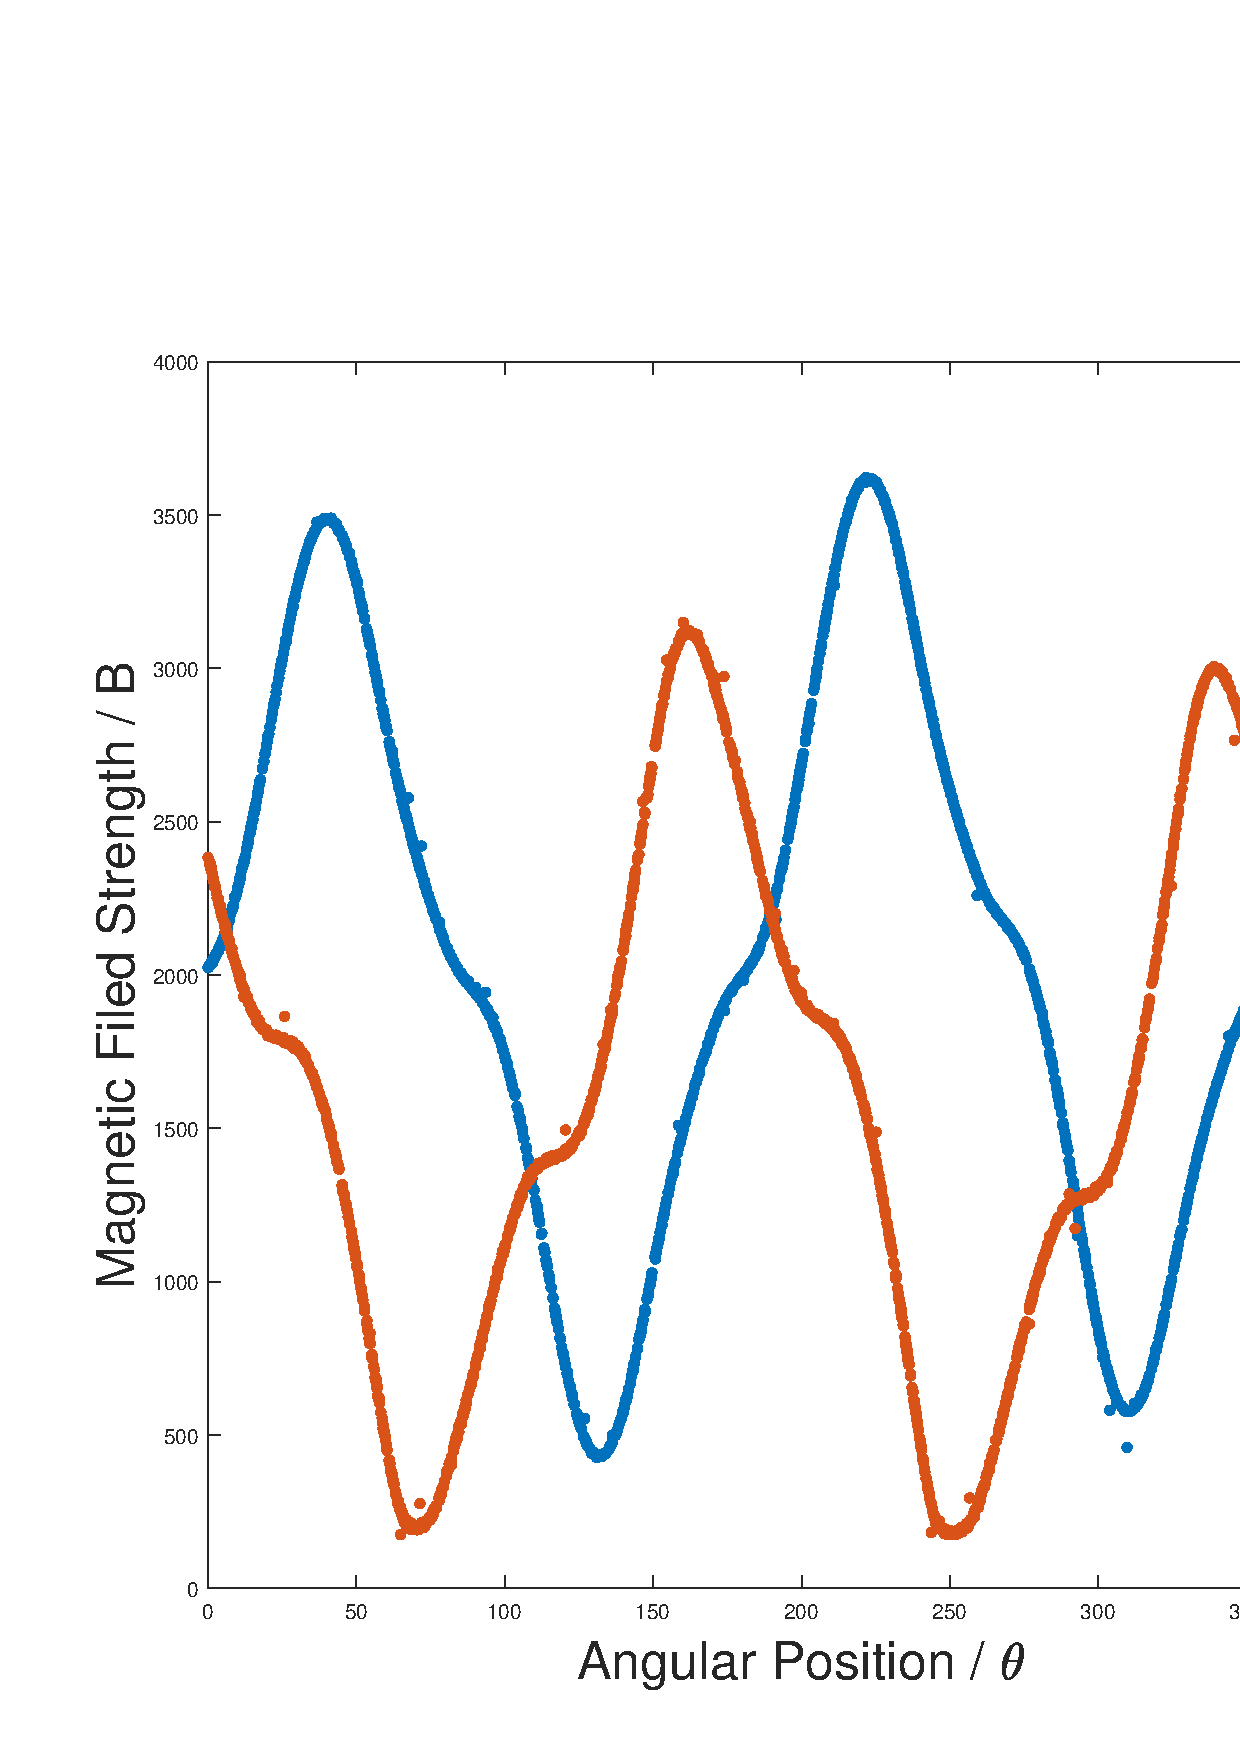
\includegraphics[width=1\textwidth]{figures/tiled_magX_vs_MagY.jpg}   		
    		\caption{Magnetic field strength with both directions in respect to the angle and with respect to each other for Position $(12\,mm, 25\,deg)$}
    		\label{fig:current pos signal shape}
    		\end{figure} 		
    		\\\\At the current position, the measurement response is comprehensible for each measurement direction as the signals $B_x$ and $B_y$ are both relatively well shaped. Regarding the left graph in Figure \ref{fig:current pos signal shape}, both curves appear to be roughly sinusoidal beside the observable signal dips. Note that the curves feature two similar cycles for one complete mechanical rotation due to the rotating two magnetic pole pairs. Therefore, observing this two cyclic nature in both signals indicates that either measurement direction obtains a decent magnetic signal from the desired magnetic field. However, the undesired curve perturbations are obviously present at this position. Assuming that both measurements are smooth sinusoidal signals, the relation between them would visualize in a two elliptic form due to the two cyclic nature. Regarding the right graph in Figure \ref{fig:current pos signal shape}, this is not the case with the current position as the perturbations clearly manifest in that representation as well. This graph provides valuable insight into the directional measurement relationship and will help understanding the respond pattern we observe at the different sensor positions. 

    		\subsection{Seeking Alternatives} \label{alternatives}
    		In the following, we present the experimental results we obtained by translating the sensor according to the given conditions we defined in the beginning of this section. Since we exclusively investigate the magnetic influences, avoiding the disturbing speed dependent sensor characteristics we mentioned in Section \ref{motivation}, is highly favourable. As this speed dependent signal transformation is negligible at lower rotation speeds, the measurements are mainly taken at a constant speed of $50\,$RPM. Furthermore, we denote the individual signal from a specific position as the \textit{position response}. \\ \\
    		To get an initial idea of the changing characteristics from different position responses, we firstly investigate the area around the original sensor position. In Figure \ref{fig:position original translated}, the results of translating the sensor $5\,mm$ along the horizontal $x_s$ axis in both directions can be observed. The blue curves represent the signal $B_x$ measured in direction $b_x$ and the orange ones, $B_y$ from measurement axis $b_y$.  Regarding the upper blue signals, we observe that beside a smaller amplitude in the right measurement, closer to the motor center, the general signal shape remains relatively similar.
    		\begin{figure}[t]
    		\begin{center}
    			\includegraphics[width=1\textwidth]{figures/Positions/original_translated_1.jpg}   
  			\end{center}
    		\caption{Measured Magnetic Signals at 3 horizontal translated Positions}
    		\label{fig:position original translated}
    		\end{figure}
	
    		In contrast to that, the change in signal $B_y$ is significant in either translation direction. The undesired shape perturbations are diminished when approaching the center of the motor while the signal gets strongly deformed at the opposite direction towards the outer motor area. To explain this discrepancy between the translated positions as well as the difference in the measurement directions, we have to take the inner architecture of the motor into account.
    		\begin{figure}[p]
    		\begin{center}
    			\includegraphics[width=0.6\textwidth]{figures/coil_distribution.jpg}   
  			\end{center}
    		\caption{BLDC Motor without the Backside Housing}
    		\label{fig:coil distribution}
    		\end{figure}
    		\begin{figure}[p]
    		\begin{center}
    			\includegraphics[width=0.8\textwidth]{figures/Positions/original_scheme.jpg}   
  			\end{center}
    		\caption{Overview of the spatial relation of the translated current position to the stator coils}
    		\label{fig:spatial relation}
    		\end{figure}
       		\\\\In Figure \ref{fig:coil distribution} the coil distribution of the BLDC Motor can be observed. The distinctions in the signal shapes are caused by different spatial relations between the measurement axes and the location of the stator coils. \\ \\
    		All three presented position responses are vertical located slightly above the stator coil $(1)$, following the enumeration from Figure \ref{fig:coil distribution}. A schematic representation of the spatial relation between the translation area and the inner motor architecture can be viewed in Figure \ref{fig:spatial relation}. To explain the obtained signals, we separately evaluate the responses with respect to the measuring direction:
    		\begin{enumerate}
    			\item According to the measurement direction $b_x$, the property $B_x$ is a measurement of the vertical magnetic field components upwards the sensor position. At the original position, the measured magnetic field is located inside the air gap between the coils $(1)$ and $(2)$ as illustrated in Figure \ref{fig:spatial relation}. When translating the position slightly in horizontal direction as we did in Figure \ref{fig:position original translated}, the sensor will still be positioned in the coil gap. Therefore, the measured magnetic field components from axis $b_x$ remain relatively similar and therefore the signal shape as well. \\ \\
    			The diminished amplitude at the more central position is related to the fact that the signal strength is proportional to the radial distance to the rotor. Hence, at the outer areas of the motor the measured magnetic signal will be the strongest.
    			\item In contrast to $B_x$, the slight horizontal position change has a crucial impact on the magnetic signal $B_y$, obtained from the measurement axis $b_y$. While $b_x$ obtains a magnetic field value upwards the sensor towards the the coil gap between $(1)$ and $(2)$, $b_y$ measures orthogonal to $b_x$ alongside the horizontal axis of the motor towards the rotor. The vertical distance of the sensor to stator coil $(1)$ is relatively small and the measurement range is limited. Therefore, the magnetic influence of the coil on the measured signal $B_y$ increases proportional to the radial distance. This affect is amplified by the orientation of coil $(1)$ as the winding distribution is not exactly symmetric towards the horizontal and vertical axis of the motor. Regarding the coil positions, coil $(1)$ e.g. is not parallel to the horizontal axis but shifted by a slight degree. Hence, the horizontal translation of the sensor at the current vertical position towards the stator, results in spatially approaching coil $(1)$ which amplifies the influence.
    		\end{enumerate}    		
    		\begin{figure}[t]
    		\begin{center}
    			\includegraphics[width=1\textwidth]{figures/Positions/original_translated_vertical_2.jpg}   
  			\end{center}
    		\caption{Measured magnetic signals at 3 horizontal translated positions, $5\,$mm below the original sensor position}
    		\label{fig:position original translated downwards}
    		\end{figure}
    	According to those conditions, the disturbance on the signal $B_y$ gets more significant when translating the sensor downwards the vertical axis $y_s$ as the distance to coil $(1)$ will decrease. In Figure \ref{fig:position original translated downwards} the responses from the similar horizontal comparison, translated $5\,$mm downwards are presented. Regarding the signal $B_y$ at the outer left position, we can hardly detect the two cyclic nature. This deformation is caused by the disturbing influence of coil $(1)$. In contrast to that, the condition of signal $B_x$ improved after the vertical translation. At the original sensor position, the measured magnetic field $B_x$ was towards the upper part of the coil gap where the deciding disturbance was in fact coil $(2)$. Moving the sensor downwards results in the measurement direction $b_x$ to approach the center of the coil gap and consequently in less magnetic disturbances.
    	\begin{figure}[t!]
    		\centering
    			\includegraphics[width=0.8\textwidth]{figures/Positions/symmetric_pattern.jpg}   	
    		\caption{Relationship between the measured signals $B_x$ and $B_y$ at several positions}
    		\label{fig:pattern}
    		\end{figure}
    	\\\\So far we investigated the area around the original sensor position. Since the stator coils are present all around the rotor, their influence can be observed at every available position. However, due to the fixed measurement directions and the shifted coil distribution we can hardly detect general response patterns. Nevertheless, we detected symmetric occurrences regarding the relation between the measurement axes. Those patterns are shifted according to the coil distribution and can be seen in Figure \ref{fig:pattern}. In this illustration, the relation between the magnetic measurements $B_x$ and $B_y$ is visualized for several positions.\\\\
    	 As mentioned earlier, if both signals would be absent of any disturbance, the graph of this relation would consist of two smooth ellipsis. Unfortunately, we did not observe such a form at any possible position. In fact, the original position still provides the best trade-off if we desire both signals to be relatively smooth. However, since the sensor features two measurement directions, the idea of utilising one signal exclusively was never considered. While additional information about the rotor is advantageous for estimating its position, using multiple measurement variables increases the complexity. The simple approach of reducing the pure number of measurement variables would already lower the complexity of the Measurement Function. But more important, when focusing on a single measurement direction exclusively we can additionally achieve a significant improvement regarding the signal condition. 
    	 \begin{figure}[t]
    		\centering
    			\includegraphics[width=1\textwidth]{figures/Positions/position_one_relation_1.jpg} 	
    		\caption{Magnetic field value $B_x$ measured at $\text{Position}_1(20\,$mm$, 4\,$deg) with spatial relation to the coils}
    		\label{fig:position one relation}
    		\end{figure}   	
    	 \\\\We observed that translating the original sensor position downwards the vertical axis towards the coil $(1)$, results in a smoother shape of signal $B_x$. Following this trend, we achieve a sensor position where the measurement $B_x$ appears to be an undisturbed sinusoidal signal. In Figure \ref{fig:position one relation} an illustration of the spatial position of the sensor as well as the responding measurement in direction $b_x$ can be observed. This position with a radial distance of $20\,$mm and an angle of $4\,$deg is located right on top of coil $(1)$. We define 
    	 \begin{equation} \label{eq:position}
    	 	Position_1 = (20\,mm, 4\,deg).
    	 \end{equation}
    	 At this position, the sensor is aligned with the coil, resulting in the measurement direction $b_x$ to measure orthogonal to the coil towards the middle of the coil gap. The influences of both coils $(1)$ and $(2)$ seem to be absent at this measurement position. A comparable good result for $B_x$ can be also achieved at the other side of the motor when mirroring this position along the vertical motor axis with a slight translation downwards the $y_s$ axis. More precisely this second alternative position is located on top of coil $(4)$ with a radial distance of $17\,$mm and an angle of $178\,$degree, 
    	 \begin{equation}
    	 \text{Position}_2 = (17\,\text{mm}, 178\,\text{deg}).
		 \end{equation}    	 		
    		\section{Considerations}
    		 The quality of the measured signal highly depends on the spatial relation between measurement axes and the stator coils. Regarding the obtained signal responses, the best way to avoid the disturbing influence of the coils is to measure exactly on top of them with a orthogonal measurement direction. According to that, the limitation in the sensor orientation change, combined with the orthogonality of the measurement directions is highly unfavourable. Those restrictions make it impossible to arrange a position where both measurement axes are orthogonal to a coil. Nevertheless, with the original position we are able to measure comparatively smooth signals in both directions even though the measured magnetic field is influenced by the stator coils. In contrast to that, if we focus on one measurement direction exclusively, namely on the signal $B_x$, we can arrange sensor positions where the measured field is in fact nearly undisturbed. Those measurement positions are located on the coils $(1)$ and $(4)$ as those are the only coils with a nearly orthogonal relation to the measurement axis $b_x$. \\\\
    		 In general, we assume that every setup can obtain a pure signal from the permanent magnets by positioning the sensor on top of an arbitrary coil. The sensor must be rotated precisely, so the according measurement axis is orthogonal to the coil orientation.\\\\    		 
    		A consideration would be, to use an additional magnetic sensor to synchronously measure at $Position_1$ and $Position_2$ in the same measurement direction $b_x$. Thus, we would obtain two sinusoidal signals out of the pure magnetic fields from the rotor without any major disturbances. Although this approach would provide ideal conditions for this estimation task, constructing an arrangement with two synchronously measuring sensors is time-consuming and induces additional costs. Therefore, we consider to use one exclusive measurement signal. If the single magnetic information about the rotor is sufficient enough to precisely estimate its position, we can utilise $Position_1$ to significantly lower the difficulty of deriving the Measurement Equation. The according Measurement Function would be univariat and sufficiently defined by a simple sinusoidal term, when neglecting the speed dependency.  \\\\
    		Another approach could be to rearrange the measurement setup in order to enable an arbitrary change in the sensor orientation. We highly suggest that with this addition, new sensor positions can be evaluated where the relation of the measurement axis to the coil is exactly orthogonal.
   
   	\chapter{Sensor Characterization - Signal Conditioning} \label{signal conditioning}
   	After providing an in-depth discussion about the shape deformation problem in the last chapter, we dedicate this chapter to the second signal distortion, namely the speed dependency. This investigation approach is purely data-driven. More precisely, we give a detailed description of the sensor output signal in order to characterize the complete manifestation of the unexpected dependency. Combined with a valuable a priori knowledge gathered from previous works, we can formulate a precise assumption on the root cause of the speed dependency. Based on this assumption, we present a new technique to approximate the unknown sensor input alongside the corresponding signal response. By processing the resulting data estimations, we gain additional insight into the measurement behaviour. Subsequently, we identify the properties of the unknown signal transformation.
 
    \section{Signal Observation} \label{signal observation}
    The measured magnetic signal itself is highly informative in terms of analysing certain signal properties. A visual analysis on the observed signal provides valuable insight into the unknown source of disturbance. In this Section we present the available display options for the measured magnetic signal and interpret the observable impact of the speed dependency.
    		\subsection{Signal Representation}\label{data representation}
    		When approaching the measured data sets, we identify mainly two essential forms of presentation that provide additional information about the signal behaviour:
    		\begin{enumerate}
    		\item Firstly, plotting the signal with respect to the sampled time steps $k$. An according graph can be seen in Figure \ref{fig:magnetic vs time}, where the magnetic signals $B_x$ and $B_y$ are presented. In this figure, the periodic nature of the signal can be clearly detected. While the shape dips are obviously present, the speed dependency can not be observed within this representation. In order to observe the manifestation of the speed dependency, we have to compare the measurements of different rotation speeds. With varying rotation speeds, the signal frequencies would diverge which makes it impossible to properly compare the signals.
			\item The other important relation we can analyse is the dependency to the angular position. An instructive visualization of this graph can be seen in Figure \ref{fig:magnetic vs angle}. In this visualisation method, the undesired speed dependency is clearly observable, as we showed in Figure \ref{fig:phase_shift_50_1000}. \\ \\
			We define this relation as
			\begin{equation}
			\begin{array}{ccl}
			f:	Rotor Angle & \rightarrow & Magnetic Field Strength \\
				     \theta & \mapsto & \begin{pmatrix}
				     B_x\\B_y
				     \end{pmatrix}	
			\end{array}	          			
			\end{equation}
			with $\theta \in [0,360)$. \\
			Ideally this dependency should be sufficiently covered by a single mapping $f(\theta)$. Unfortunately, due to the speed dependency this mapping is unique for every possible rotation speed $\omega$.
    		\end{enumerate}
    		\begin{figure}[p!]
    		\begin{center}
    			\includegraphics[width=1\textwidth]{figures/Time_200rpm.jpg}   			
  			\end{center}
    		\caption{Measured magnetic field strength in both direction vs time at $200\,$RPM}
    		\label{fig:magnetic vs time}
    		\end{figure}
    		\begin{figure}[p!]
    		\begin{center}
    			\includegraphics[width=1\textwidth]{figures/Angle_200rpm.jpg}   			
  			\end{center}
    		\caption{Measured magnetic field strength in both direction vs rotor angle in Degree at $200\,$RPM}
    		\label{fig:magnetic vs angle}
    		\end{figure}
    		\subsection{Speed Dependency} \label{speed dependency}
    		The observable speed dependency manifests mainly as a phase shift, proportional to the rotation speed. Beside this phase shift, when surpassing a certain speed of approximately $2000\,$RPM, the signal amplitude is diminished significantly. A comparison of the magnetic signal at a velocity of $200\,$RPM versus a signal at $3000\,$RPM clearly illustrates those two occurrences and can be seen in Figure \ref{fig:200RPM vs 3000RPM}.
    		\begin{figure}[t]
    		\begin{center}
    			\includegraphics[width=1\textwidth]{figures/phaseshift_200_3000.jpg}   		
  			\end{center}
    		\caption{Magnetic field strength vs angular position at $200\,$RPM and $3000\,$RPM}
    		\label{fig:200RPM vs 3000RPM}
    		\end{figure}
    		\begin{figure}[t]
    		\begin{center}
    			\includegraphics[width=1\textwidth]{figures/phaseshift_neg_200_3000.jpg}   		
  			\end{center}
    		\caption{Magnetic field strength versus angular position at $-200\,$RPM and $-3000\,$RPM}
    		\label{fig:neg 200RPM vs 3000RPM}
    		\end{figure}
    	Note that for presentation purpose only one direction of the measurement is shown. However, those anomalies reveal in both measurement axes in nearly the same extent. Regarding the signal measured at $3000\,$RPM, what stands out is that the curve dips which are clearly present in the $200\,$RPM curve, seem to be almost disappeared at the higher rotation speed. This curve smoothing trend appears alongside the mentioned amplitude diminishing, starting upon a certain threshold. \\\\
    	In contrast to the shown response at positive rotation, the observable signal transformation is even more significant at the opposite rotation direction. While the amplitude diminishing threshold is approximately even, the extent of transformation when surpassing this point is noticeably stronger in negative rotation direction. Especially the curve smoothing behaviour at higher signal frequencies can be clearly detected in measurements at this rotation direction. In Figure \ref{fig:neg 200RPM vs 3000RPM}, a similar comparison as the previous is shown for the opposite rotation direction. The observed signal at a velocity of $-3000\,$RPM appears to be a smooth sine wave. \\\\
    		Due to this diminishing behaviour above a certain threshold as well as the general speed proportional signal shaping, we highly suggest that the sensor acts as an interfering low-pass filter. According to this assumption, the measured signal $y(k)$ emerges out of a convolution between the original signal $u(k)$ and the unknown filter function $h(k)$ as
    		\begin{equation}
				y(k) = h(k)*u(k).\label{eq:convolution}   		
			\end{equation}
		If this assumption is correct, the original signal $u(k)$ would be absent of any speed dependency. Unfortunately, we have neither access to this signal nor any further information about its properties beside our suggestions and the measured output signal $y(t)$. 			
    
    \subsection{Coilless Measurements} \label{coilless measurements}
    	In \cite{mayerposition} an experimental setup was constructed, where the motor housing including the stator coils was detached from the motor. The goal of this approach was to gather further information about the extent of influence the stator has on the measured magnetic field. The sole rotor was driven by an external driving motor to produce the necessary rotation of the permanent magnets. The magnetic measurement response of this setup is as expected a smooth sinusoidal signal in both measurement directions. A representation of these measurement can be observed in Figure \ref{fig:coilless signal overview}.
		\begin{figure}[t]
    		\begin{center}
    			\includegraphics[width=1\textwidth]{figures/coilless_signal_overview.jpg}   
  			\end{center}
    		\caption{Signal presentation of the coilless measurements at $500\,$RPM in either measurement direction}
    		\label{fig:coilless signal overview}
    		\end{figure}
    		\begin{figure}[t]
    		\begin{center}
    			\includegraphics[width=1\textwidth]{figures/coilles_phase_shift.jpg}   
  			\end{center}
    		\caption{Demonstration of the phase shifting occurrence at different rotation speeds and directions for both measured signals}
    		\label{fig:coilless signal phase shift}
    		\end{figure}  
    	 While the signal shape is completely absent of disturbing influences, the speed dependency is still present in the coilless observations. The transformation can be observed in either measurement axis $b_x$ and $b_y$ as well as in both rotation directions. In Figure \ref{fig:coilless signal phase shift} the speed proportional phase shifts are demonstrated for rotational speeds in opposite directions. Note that the amplitude diminishing effect we observed upon a certain threshold of approximately $2000\,$RPM, is not observable within this setup as the external driving motor is limited to a rotation speed of $\approx1500\,$RPM. \\\\
    	Since the speed dependent distortions are still clearly observable in this exclusive setup, this occurrence can only be directly caused by an unknown sensor function. We can utilise the coilless data to approach an exclusive investigation on this unknown frequency response, without any uncertain influences from the stator coils.
   
    	\section{Data Preparation}\label{data preperation}
    	So far we observed an omnipresent speed dependent signal transformation. Even in the previous discussed coilless experiment, where the only influencing factors are the measuring sensor including the corresponding electronics and the signal producing rotor itself, we can obviously detect this effect. In this section we will present a technique to estimate the original speed independent signals. This simulation technique provides the foundation for a complete sensor characterization.
    		\subsection{Assumption}
    	According to the sensor assumption, every measurement 
    	\begin{equation}
 			y_k = \begin{pmatrix}{B_x}_k\\{B_y}_k\end{pmatrix}
		\end{equation} 			
 			 at an arbitrary time point $k$, is the result of a convolution between the original speed independent signal $u_k$ with an unknown sensor function $h(.)$ as in \eqref{eq:convolution}. The measured output $y_k$ alone is not sufficient enough to characterize the properties of the function $h(.)$, as this output could result out of any arbitrary input. Therefore, we have to gather additional informations about the original signal $u_k$. \\\\
 			 Regarding the graphs presented in Figure \ref{fig:coilless signal phase shift}, we observe that the signals at the small rotation speed of $150\,$RPM, are exactly positioned in the center of the higher speed measurements. This pattern can be detected through all measurements as an increasing rotation speed proportionally amplifies the occurring shift. This condition perfectly matches the nature of a low-pass filter. The general behaviour of such filters is, that low frequency signals can pass unhindered while higher frequency will be phase shifted as well as diminished \cite{tietze2013halbleiter}. \\ \\
    		Under this consideration, we highly suggest that the nature of the original signal $u_k$ is similar to the signal behaviour at low rotation speeds. The resulting idea is, to transfer the nature of the comparably unaffected low speed measurements to higher frequencies.  The result is an estimation $\hat{u}_k$ of the original magnetic field value $u_k$. Note that in the following we will reference the actual measurement $y_k$ as the output and the unbiased signal $u_k$ as the input, according to the convolution equation \ref{eq:convolution}. \\ \\
    		To accurately characterize the unknown filter function $h(.)$, we require both the output and the input at several coherent time points $k$. Additionally, these pairs must we produced by the exact same rotor state. More precisely, if we consider a data set with a quantity of $K$, in every \textit{input}-\textit{output} pair $(u_k,y_k)$ with $k\in\{1\dots K\}$, both values have to relate to the exact same rotor angle $\theta_k$ in order to comprehend the transformation. We describe these ideal \textit{input}-\textit{output} pairs as
    		\begin{equation}\label{eq:input-output pair}
    		({u_\theta}_k,{y_\theta}_k).
    		\end{equation}
    		The in the next section presented technique, allows to estimate these desired value pairs for arbitrary velocities in either rotation direction.
    		\subsection{Input Approximation} 		
    		Firstly, we have to simulate the angle sequence the rotor traverses through when rotating at a specific rotation speed. Additionally, the angle sequences must be simulated with respect to the sampling time $\Delta T$. This simulation has the purpose to obtain a set of angular positions which represent the motor rotation at constant velocities. In terms of the simulation, these angle sequences will be the rotor states which produce the desired magnetic \textit{input}-\textit{output} values.\\\\
    		Suppose we want to generate $N$ \textit{input}-\textit{output} value pair approximation $(\hat{{u_\theta}}_n,\hat{{y_\theta}}_n)$ for a constant velocity $\omega$. Therefore, we sample the according angle sequence by calculating
    		\begin{equation}
    			\theta_n = (n * \Delta T * \omega) \mod 360,
    		\end{equation}
    		for every time point $n = 1 \dots N$, with the sampling time $\Delta T = 0.0022$ and the speed $\omega$ in \textit{Degrees Per Second}. Subsequently, we have to  map these generated angle sequences on the individual magnetic signal values. To achieve this, we utilise the in Section \ref{data representation} presented dependency
    		\begin{equation}
			\begin{array}{ccl}
			f:	Rotor Angle & \rightarrow & Magnetic Field Strength \\
				     \theta & \mapsto & \underline{B}.
			\end{array}	          			
			\end{equation} 
    		Since the signal depends on the rotation speed, this function is unique for every velocity $\omega$. Accordingly, we define the speed specific relationship  as 
    		\begin{equation}
    		f_\omega(\theta) = \begin{pmatrix}
    		B_x\\
    		B_y
    		\end{pmatrix}.
    		\end{equation}
    		Thus, to transfer the desired signal nature of a low rotation speed $\omega_l$ to a higher velocity $\omega_h$, we have to mathematically define the two functions ${f_\omega}_l$ and ${f_\omega}_h$. As the setup allows us to gather datasets of arbitrary size and speed, we firstly take two separate measurements at the according rotation speeds $\omega_l$ and $\omega_h$. The quantity of the obtained datasets has to be long enough to clearly represent the speed specific signal behaviour. With those measurements, the definition of ${f_\omega}_l$ and ${f_\omega}_h$ can be derived by applying appropriate regression techniques. In case of the coilless measurements we derived the functions with a \textit{Sum of Sine Model} provided by the \textit{Curve Fitting Toolbox} \cite{matlabcurve}. Note that the complexity of these functions has no impact on the general estimation complexity since this procedure is performed within the Offline mode and therefore does not directly effect the on-time estimation. \\ \\
    		To complete this approach, we apply both of the defined relations ${f_\omega}_l$ and ${f_\omega}_h$ on the previously derived angle sequence $\theta_n$. The results are $N$ of the desired \textit{input}-\textit{output} approximations $(\hat{{u_\theta}}_n,\hat{{y_\theta}}_n)$. We describe this last step as 
    		\begin{equation}
    		\begin{aligned}
			{f_\omega}_l(\theta_n) &=  \underline{B}_n^l = \hat{{u_\theta}}_n		 \\
			{f_\omega}_h(\theta_n) &=  \underline{B}_n^h = \hat{{y_\theta}}_n,
			\end{aligned}
    		\end{equation}
    		for $n = 1\dots N$.
    		\begin{figure}[t]
    		\begin{center}
    			\includegraphics[width=1\textwidth]{figures/block_diagram_sampling.jpg}   
  			\end{center}
    		\caption{Blockdiagram of the input approximation technique}
    		\label{fig:input estimation}
    		\end{figure}
    		\\\\To give an overview of this combined \textit{input}-\textit{output} approximation technique, in Figure \ref{fig:input estimation} an exemplary illustration of the whole procedure is given. In this example we generate the value pairs for a rotation speed of $1000\,$RPM by using the signal behaviour from a $150\,$RPM measurement as the input reference. The result of the presented example can be see in Figure \ref{fig:input output time}, where both the estimated \textit{input} and \textit{output} for signal $B_x$ are shown in respect to the measurement time points $k$. Regarding the condition of the signals, we successfully transferred the unaffected signal behaviour of a low speed measurement on a higher frequency. Hence, we can now observe the manifestations of the filter function with respect to the time.
    		\begin{figure}[t]
    		\begin{center}
    			\includegraphics[width=1\textwidth]{figures/input_output_time_final_1.jpg}   
  			\end{center}
    		\caption{Result of the input-output simulation at a speed of $1000\,$RPM}
    		\label{fig:input output time}
    		\end{figure}
    		\\\\We can apply this technique on every measurable speed with an appropriate input reference. This enables the opportunity to precisely compare the extent of signal transformation between different velocities. Therefore, this estimation technique will be the base for the further sensor characterization as well as the fundamental source for the System Identification approach we present in Chapter \ref{system identification}. 
   	\section{Frequency Analysis} \label{frq analysis}
   			We identified that the used Honeywell sensor features an unknown function $h(.)$. Commonly such a signal transforming instance is called a $System$. A block diagram of the sensor system is shown in Figure \ref{fig:block diagram sensor system}. The characterization of unknown systems is an important task in various application fields, involving signal processing hardware. A common approach is to investigate the signal in the frequency domain to gain additional information about the system dynamics as such transformation features many advantageous properties.
   			\begin{figure}[t]
    		\begin{center}
    			\includegraphics[width=0.8\textwidth]{figures/block_diagram_convolution.jpg}   
  			\end{center}
    		\caption{Block diagram of the sensor system}
    		\label{fig:block diagram sensor system}
    		\end{figure}
   			 \\\\While in time domain the sensor system involves an unknown convolution, this relation becomes a simple multiplication when transforming the signals into the frequency domain \cite{roberts2020signals}. Consider a linear time-invariant system, when performing a Laplace transformation on both signals as $\mathcal{L}\{u(t)\} = U(s)$ and $\mathcal{L}\{y(t)\} = Y(s)$ with the complex variable $s$, the time domain system equation
   			\begin{equation}
   			y(t) = h(t)*u(t)
   			\end{equation}
   			becomes
   			\begin{equation}
   			Y(s)=H(s)X(s).
   			\end{equation}
   			The Laplace transformed system function $H(s)$ is called \textit{Transfer function} and can be defined by the ratio of the Laplace transformed input and output,
   			\begin{equation}
   			 H(s) = \frac{Y(s)}{U(s)}.
   			\end{equation}
   			Unfortunately, in the dynamic sensor system, the signal filtering highly depends on the specific signal frequency. Therefore, deriving this Laplace transformed input-output ratio would exclusively describe the relation between the individual given input-output pair. Nevertheless, we can still gain additional information out of the frequency domain by analysing the system's \textit{Frequency Response}.\\ \\
   			A popular characterization approach is, to analyse the system response to different frequencies. Therefore, the system is usually excited by sinusoidal signals at various frequencies to measure the according system output, which is called the Frequency Response. Comparing the response signal with the according input in frequency domain, provides valuable details about the amplitude and phase transformation. In the sensor system, the common approach is not applicable since the function $h(k)$ is unknown and injecting the system with arbitrary inputs is not available. However, due to the periodic nature of the signal and the changing frequencies, the regular setup operation already performs such a system excitation. In fact, the generated \textit{input}-\textit{output} approximations present an ideal base for this frequency domain investigation technique. \\ \\
   			David C. Rife (2020) \cite{roberts2020signals} presented a method to estimate the parameter of discrete noisy data at a constant frequency. The basic idea is to perform a \textit{Discrete Fourier Transformation} and subsequently estimate the amplitude values with an \textit{Maximum Likelihood Estimation}. Since our generated \textit{input}-\textit{output} approximations are in fact discrete data sets with a common frequency, we can apply this technique to calculate the amplitude and phase ratios for every sampled velocity. Thus, we utilised a Matlab implementation based on this approach to characterize the amplitude and phase transformation in respect to the according frequencies. This implementation is provided by \cite{matlabamplitude}. \\ \\
   			The obtained frequency response from the coilless measurements was in fact a characteristic low-pass response. The calculated phase shift value in Degree constantly increased alongside the rising rotation speed and the amplitude was slightly diminished at higher frequencies. While the coilless data provides the purest sensor behaviour, the restricted velocity at a maximum of $1500\,$RPM crucially limits the integrity of this characterization approach. This condition is amplified by the fact that low-pass filter mainly reveal their influences at higher frequencies. Therefore, we applied the similar approach to measurements from the original sensor position. The speed range is from $50\,$RPM up to $4000\,$RPM. The resulting amplitude and phase discrepancies are visualized in Figure \ref{fig:bode}, where those ratios are shown in respect to the according rotation speed in $ln(\omega_{RPM})$.
   			\begin{figure}[p]
    		\begin{center}
    			\includegraphics[scale=0.22]{figures/bode.jpg}   
  			\end{center}
    		\caption{Amplitude and phase ratio in respect to the signal frequency}
    		\label{fig:bode}
    		\end{figure} 
    		\begin{figure}[p]
    		\begin{center}
    			\includegraphics[width=1\textwidth]{figures/bode_reference.jpg}   
  			\end{center}
    		\caption{Frequency response of a two-order low-pass filter, adopted from \citep{liang2008study}}
    		\label{fig:bode reference}
    		\end{figure}
   		\\\\Regarding this graph, we can clearly observe a speed proportional negative phase shift as well as a diminished amplitude upon a certain cutoff frequency. As this frequency response features all the common low-pass characteristic, we can confidently say that our prior suggestion was correct. To provide a comparison, in Figure \ref{fig:bode reference} the Bode diagram of a typical low-pass filter can be observed. Comparing these two frequency responses, the similarities in both properties are indisputable. 
    \chapter{System Identification} \label{system identification}
    	In the previous chapter we identified the source of the speed dependency, namely the sensor and involved electrical components. Hence, spatial changes or any rearrangements will neither influence the presence of this occurrence nor diminish the extent of disturbance. In order to eliminate the undesired property of the sensor measurement, we need to condition the measured output signal. \\\\
    	In this chapter we present the approach of eliminating this undesired transformation by post-processing the measured magnetic field signals. Thus, we begin by discussing the filter function in context of the Online estimation. Subsequently, we present the idea of a "deconvoluting" system. Finally, the chosen identification techniques are briefly described. 
    	\section{Online Estimation}
    	Ideally, we would describe $f$ by a simple equation, mapping the angular position $\theta$ on the speed independent sinusoidal signal $u_k$. However, the only available measurement during the estimation is in fact the corrupted output signal
    		\begin{equation}
    			y_k = h * u_k + v_k.
    		\end{equation}
    		This condition is illustrated in Figure \ref{fig:classification sensor system}, where a block diagram of the estimation model including the sensor system is presented. 
    		\begin{figure}[t]
    		\begin{center}
    			\includegraphics[width=1\textwidth]{figures/sensor_system_online_2.jpg}   
  			\end{center}
    		\caption{Overview of the Online estimation model including the sensor system}
    		\label{fig:classification sensor system}
    		\end{figure}
    		According to that, the implemented Measurement Function must define a mapping of the predicted system states $\underline{x}_k^p$ on the filtered magnetic field values $y_k$. Our goal is to produce a speed independent measurement variable $\hat{u}_k$.\\\\
 			
    	\section{Deconvoluting System}
    	The fundamental idea is, to construct an additional system $g$ which subsequently processes the convoluted measurement $y_k$. The output of this system shall be a speed independent magnetic field value with an exclusive dependency to the rotor's position. Ideally, the output of this system $g$ would be the original undisturbed magnetic signal $u_k$. Since in practise no system will be able to reconstruct the exact unconvolved signal $u_k$, we seek a system that responds with an optimal estimation $\hat{u}_k$. Accordingly, we define the equation of the desired system $g$ as
    	\begin{equation}
    	\hat{u}_k = g * y_k = g * h(u_k).
		\end{equation}    	
	To give an overview of our approach, in Figure \ref{fig:deconvolution system} a block diagram of these two involved systems is presented. The Figure illustrates the relation between the undisturbed signal $u_k$, the actual measurements $y_k$ and the estimated signal $\hat{u}_k$ in context of the sensor and "deconvoluting" system. \\\\
		The difficulty of constructing such a specific system is the missing knowledge on the desired signal $u_k$. The measurements $y_k$ and our previous obtained characterization are the only available information concerning the filter behaviour. The process of defining a mathematical description for a system, based on pure observations is termed as \textit{System Identification} \cite{sid}.
		\begin{figure}[t]
    		\begin{center}
    			\includegraphics[width=1\textwidth]{figures/deconvolution_system.jpg}   
  			\end{center}
    		\caption{Overview of the "deconvoluting" system idea}
    		\label{fig:deconvolution system}
    		\end{figure} 
    	\subsection{Special Conditions}
    	In Chapter \ref{theoretical background} we briefly discussed the fundamental concept of this study. Most System Identification application will validate an identified model mainly on its capability of reproducing the desired system behaviour. In contrast to that, our identification approach requires deviating satisfaction criteria such as the system complexity and quantity of required systems. Additionally, we encounter specific conditions such as missing comparability and unavailable knowledge about the output signal, which both complicate this task significantly.
    	\subsubsection{Comparability}
    	The most significant distinction in contrast to common approaches is, that the desired system $g$ does not exist. More precisely, we aim to construct a system model that inverts the transformation performed by another system. Since the sensor system is unknown, the obvious approach of simply deriving the inverse of this filter function would involve the study of \textit{Blind Deconvolution}. These techniques require to assume many crucial system properties a priori \cite{489268}. In Chapter \ref{signal conditioning} we already identified certain system properties and developed a method to approximate the system inputs. These prepared data pairs provide an ideal base for a suitable System Identification technique. Therefore, directly constructing a "deconvoluting" system  based on the data approximations requires no additional assumptions. \\\\
    	The downside of our implementation approach is the validation. We can not compare the output of the identified system with the real measurement responses since $u_k$ is unknown. Nevertheless, we can still decide if an obtained model sufficiently describes our desired dynamics based on three validation techniques:
    	\begin{enumerate}
    		\item Using the approximated \textit{input}-\textit{output} pairs obtained by the presented data simulation technique. The identified systems will be based on such estimated data sets. However, these pairs can additionally be used to subsequently validate the constructed models. We can inject the identified model with the output signal estimation $\hat{y_k}$ and compare the response with the according input approximation $\hat{u_k}$. By using independent measurements to generate them, we can increase the integrity of this validation approach. 
    		\item The second method is a visual comparison with real measurements using the angular positions. When exciting the identified system with observations from higher rotation speeds, the relation of the response to the angular position can be analysed. Ideally, this relation should be similar to measurements of low velocities. An identified system successfully models the desired dynamics, if the speed dependent phase and amplitude transformation can not be detected at the output anymore. 
    		\item Finally, we can observe the estimation results. Since the purpose of the identified models is to be integrated in the estimation task, we can simply implement the systems into the online estimation. The models are then validated by observing the estimation performance.
    	\end{enumerate}
    	
    	\subsubsection{Complexity}
    	While we can utilise these alternative validation methods to analyse the fit of the identified systems, we have to consider the system complexity. Our desire is to reduce the complexity in the overall estimation task. Therefore, a system that produces precise estimation results but only under the premise of a significant complexity is highly unfavourable. Hence, this identification task requires a system that models a trade-off of these two criteria.
    	\subsubsection{Quantity}
    	So far we discussed the challenge of constructing a single deconvoluting system. In fact, the number of required models is proportional to the dimension of the used measurement vector. While we briefly mentioned the consideration of implementing a single measurement dimension, the common approach of this task involves both measurement axes. When utilising both magnetic signals $B_x$ and $B_y$, we need two systems to post-process each signal individually. \\\\
    	Additionally, we have to consider the signal distinction between the different rotation directions. We could probably construct a single system, capable to process the signal of both rotational direction. Unfortunately, such a model would involve a significant complexity. Therefore, we will identify an additional system for the opposite rotational direction. Each model is then applied separately according to the current rotational direction. 
		\subsubsection{Data}
    	 The most obvious challenge in this task is the lack of output knowledge. The unknown signal $u_k$ is in terms of the desired system $g$ the ideal output. To solve this knowledge problem, we use the presented data simulation technique to gather the approximated \textit{input}-\textit{output} of the sensor system. These pairs are then used the other way around to model the desired system. More precisely, the simulated response of the sensor system $\hat{y}_k$ represents the input for the system identification. The approximation of the original signal $\hat{u}_k$ is the system output. The identified model shall then reproduce this output when exciting it with real measurements $y_k$. Hence, the used data estimation pairs must be generated wisely as their relation has to define the complete sensor system characteristic.
    	\subsection{Offline Preperation}	
    	In previous works, the task implemented in the Offline step consisted mainly of regressing and validating efficient measurement functions. With the presented deconvoluting system approach, the procedure is expanded with two additional tasks. Firstly, preparing the estimated data pair sets and secondly, obtaining the "deconvoluting" system. Following the data simulation technique from Section \ref{data preperation}, the first step is to chose an appropriate low speed reference behaviour. This behaviour is then transferred on every relevant frequency to obtain the outputs $\hat{u}_k$. The role of the reference signal is crucial since the identified system will produce an estimation of this exact observable signal behaviour. Therefore, the mathematically defined relation between this reference signal and the angular position will simultaneously be used as the Measurement Function. To illustrate that interaction between the Measurement Function and the System Identification, in Figure \ref{fig:offline sid} we present an overview of the new Offline estimation procedure.
    	 \begin{figure}[p]
    		\begin{center}
    			\includegraphics[width=1\textwidth]{figures/offline_sid_1.png}   
  			\end{center}
    		\caption{Overview of the Offline procedure including the System Identification }
    		\label{fig:offline sid}
    		\end{figure}
    	\section{Identification techniques}
    	According to the System Identification loop in Figure \ref{fig:sid loop}, we selected a set of three identification techniques, that we present in this section. These specific algorithms were chosen as they represent a different fundamental concepts of System Identifcation approaches. More precisely, the first technique identifies the system characteristics purely on time domain analysis. The second approach utilises a Laplace transformation to model the desired dynamics. The final method identifies the properties through \textit{Subspaces} and consequently trains a state space system equation. We used the Matlab implementation of these techniques provided by the System Identification Toolbox \cite{ljung1995system}.\\\\
    	Note that in our application, the system input is in fact the sensor output $y_k$. For convention purposes, we term the input of the identified system as $u(t)$ and the responding output as $y(t)$, with respect to time $t$. We will only present the basic concepts of these approaches and discuss their drawbacks. For further information about the implementation details, we reference to the according literature. 
    	\subsection{Correlation Analysis} \label{imp}
    	A linear discrete-time system can be described by its \textit{Impulse Response} $g$ as 
    	\begin{equation}
    	y(t) = \sum_{k = 1}^{\infty}g(k)u(t-k)+v(t)
    	\end{equation}
    	with disturbance $v(t)$ \cite{ljung1999system}. Assuming the input $u(t)$ as well as the noise $v(t)$ to have zero mean and be uncorrelated to each other, the cross correlation function $R_{uy}$ can then be described as
    	\begin{equation}
    	R_{uy}(\tau) = \sum_{k = 1}^{\infty}g(k)R_u(k - \tau),
    	\end{equation}
    	for an impulse $\tau$. The idea is to approximate the cross correlation function $\hat{R}_{yu}$ as well as the auto correlation $\hat{R}_u$. Hence, for a finite number $N$, the system is treated as a Finite Impulse Response model of order $N$. The characterizing parameters can then be derived by solving the equation
    	\begin{equation}
    	\hat{R}_{uy} = \sum_{k = 1}^{N} g(k)\hat{R}_u(k - \tau). 
    	\end{equation}
    	The difficulty of this derivation decreases significantly if the input signal is white noise, therefore this algorithm commonly uses a prior whitening filter. \\ \\
    	This technique is straight forward as no assumptions about the model parameters or possible structures have to be taken a priori. The dynamics can simply be modeled by exciting the system with a finite set of input variables. This finite nature simultaneously induces the most significant drawback of this approach. To model the complete characteristic of a system, this finite input set has to be large enough to contain the desired dynamics. The problem is that the quantity of these finite observations is equal to the order of the resulting system. Therefore, using large data sets lead to a significant model complexity. On the other hand, applying too short input sets will not be sufficient enough to estimate the entire system dynamics. 
    	\subsection{Instrumental Variable Estimation} \label{SRIVC}
    	Consider a linear continuous-time system described by its differential equation as in \eqref{eq:differential}. This definition can be rearranged to following structure 
    	\begin{equation}
    	y(t) = \frac{b_0s^m + b_1s^{m-1} + \cdots + b_m }{s^n + a_1s^{n-1} + \cdots + a_n} u(t),
    	\end{equation}
    	with $s$ as the differential operator. The idea of the algorithm, termed \textit{Simplified Refined Instrumental Variable Method} (SRIVC) is, to assume the fraction in this equation to be the Laplace transformed transfer function according to \eqref{eq:transfer function}. By utilising the linearity of the system, the equation be can rearranged in a form where both the input and the output are multiplied with $\frac{1}{A(s)}$ \cite{young2006optimal}. The next step is to pre define this filter $\frac{1}{A(s)}$ and derive the Inverse Laplace Transformation 
    	\begin{equation}
    	\mathcal{L}^{-1}(\frac{s^i}{A(s)}),
    	\end{equation}
    	for $i = 1 \cdots n$ and $i = 1 \cdots m$. Hence, a proper error function can be constructed which describes the base for a maximum likelihood estimation. Thus, an estimation of the desired parameter vector 
    	\begin{equation}
    	\theta = [a_0 \dots a_n \, b_0 \dots b_m], 
		\end{equation}
		is obtained. \\ \\
		This technique is a simplified form of the \textit{Refined Instrumental Variable Method} as this approach assumes white noise. The main drawback of this technique is that the filter $ F = \frac{1}{A(s)}$ as well as the model order have to be approximated a priori. When these values are initialised properly, the algorithm provides an efficient system model by iterative refining the system and filter parameters. Nevertheless, due to the iterative nature the approach can suffer from convergence problems. 
    	\subsection{Subspace Identification} \label{n4sid}
    	In contrast to the previous presented technique, the non-iterative \textit{N4SID} (Numerical algorithm for Subspace State Space System Identification) algorithm provides a guaranteed convergence \cite{van1994n4sid}. This approach describes the system in a state space form as in \eqref{eq:state space}. Note that for simplicity the system and measurement noise are neglected. The base for this technique is to define a set of \textit{Block Hankel Matrices} containing the values of "past" and "future" inputs/outputs. The main step is to project the "future" inputs along the row space of the "future" outputs into the row space of the "past" in- and outputs. Thus, the matrix $Z_i$ is obtained with $i$ as the \textit{prediction horizon}, which represents the cut-off between the "past" and the "future". The sub-spaces of this matrix contain the valuable information about the system parametrization as well as the model order. By deriving a \textit{Singular Value Decomposition}, the so called \textit{extended controllability matrix} $\Gamma$ is obtained, which defines
    	\begin{equation}
    	\Gamma_i = \begin{pmatrix}C \\ CA \\ CA^1 \\ \vdots \\ CA^{i-1}\end{pmatrix}.
    	\end{equation}
    	Based on $\Gamma$, the parametrization of the system matrices $A$,$B$,$C$ and $D$ can be estimated \cite{jamaludin2013n4sid}. \\ \\
    	The major advantage of this technique is that neither prior assumptions about the model order nor any initial parametrization have to be defined. These properties are both estimated out of the subspaces of the mentioned projection.
  	\chapter{Evaluation}\label{evaluation}
  	In this chapter, we evaluate the presented approaches. The main goal is to validate the performance of the identified "deconvoluting" systems in the Online estimation procedure, presented in \ref{estimation approach}. Firstly, we discuss the identified systems in general. We evaluate their capability of reproducing the desired signal behaviour by using a visual comparison and a suitable error metric. This metric is the Root Mean Squared Error (RMSE), defined as   
  		\begin{equation}
  		RMSE = \sqrt{\frac{1}{N}\sum_{i=1}^N(\hat{u}_i - u_i})^2, \label{eq:rmse}
  		\end{equation}
  		with the system output $\hat{u}_i$ and the ground truth signal $u_i$. Subsequently, the new estimation approach is validated using the coilless data with both signals $B_x$ and $B_y$. The final evaluation addresses the new sensor position $Position_1$, elaborated in Section \ref{alternatives} and the "deconvoluting" systems from Chapter \ref{system identification}. This technique combines both disturbance elimination approaches. Thereby, we additionally evaluate the idea of using a single measurement axis $b_x$ exclusively. \\\\
  		In general, the tested data sets cover a speed range of $-1500\,$RPM to $+1500\,$RPM. We separately use two different measurements: 
  		\begin{enumerate}
  			\item From the coilless setup with both measured signals $B_x$ and $B_y$.
  			\item An exclusive measurement $B_x$, observed at $Position_1$. This set is obtained from the regular motor setup, including the stator coils. 
  		\end{enumerate}
  		\section{System Identification} \label{evaluation sid}
  		As mentioned in Chapter \ref{system identification}, the Online estimation approach requires at least two "deconvoluting" systems. A system $g^+$ for positive rotation direction and the other $g^-$ for the negative case. If both measurement signals are considered,  these system pairs are required for either signal. \\\\We refer to the three identification techniques as \textit{Imp} (Impulse Response Model), \textit{SRIVC} (Simplified Refined Instrumental Variable Method) and \textit{N4SID} (Numerical algorithm for Subspace State Space System Identification).
  		\subsection{Performance on Simulated Data}
  		In this section we evaluate the performance of the "deconvoluting" systems on the approximated input-output pairs. The used test sets are simulated from an independent measurement to increase the integrity of the validation. The error is derived by injecting the constructed systems with the approximation $\hat{y}_k$ and comparing the system output with the corresponding approximation $\hat{u}_k$. 
  		\subsubsection{Coilless}
  		We chose the lowest available speed of $150\,$RPM as reference input for the coilless data. Since in this case, both measurement axes are considered, we identified four different systems with each identification technique.\\\\
  		 In Table \ref{table:sid results coilless} the RMSE for five different rotation speeds in each rotation direction are shown. Note that in this table only the results for $B_x$ are presented since the errors on $B_y$ are comparable. The similar comparison for signal $B_y$ can be found in Appendix \ref{appendix:sid results coilless}.  Regarding the error over all speeds, the \textit{N4SID} model clearly provides the best system modeling.
  		  With an average RMSE of $17.0849$, the \textit{N4SID} systems precisely model the desired system dynamics. Nevertheless, the output of the other two models is still precise if we consider the value range of the magnetic measurements. The magnetic signal $B_x$ in this test set features a minimum of $441$ and a maximum of $3643$. We observe the \textit{SRIVC} models perform as good as the \textit{N4SID} on positive rotation directions. However, in the opposite rotation direction, the error of the \textit{SRIVC} increases significantly. In contrast to that, the \textit{Imp} and \textit{N4SID} models perform constantly for both rotation directions. \\\\  	 		  Beside the rotation direction, we can observe an increasing error trend with faster rotation speeds. Especially the $\textit{SRIVC}^-$ has a noticeably increased RMSE at high negative velocities. The model produces the highest error in this comparison of $103.7956$ at the speed of $-1500\,$RPM. This trend is comprehensible as the extent of required signal transformation is proportional to the signal frequency. More precisely, the "deconvoluting" systems revert the signal transformation performed by the sensor's low-pass filter. Since this transformation is more significant at higher rotation speeds, the difficulty of reverting this behaviour increases as well. 
		 \begin{table}[t!]
		 \centering
	\begin{tabular}{|c|c|c|c|}

	\hline
	\multicolumn{4}{|c|}{\textbf{RMSE($B_x$)}}                        \\ \hline\hline
	\textbf{}            & \multicolumn{3}{c|}{\textbf{System Model}} \\ \hline
	\textbf{Speed / RPM} & \textbf{Imp}          & \textbf{SRIVC}         & \textbf{N4SID}       \\ 		\hline
	+500                 & 27.4521      & 17.8709       & 17.8048     \\ \cline{1-1}
	+800                 & 30.9390      & 12.4576       & 11.9217     \\ \cline{1-1}
	+1000                & 31.0857      & 14.0665       & 13.3447     \\ \cline{1-1}
	+1200                & 37.5183      & 17.7959       & 17.4107     \\ \cline{1-1}
	+1500                & 56.5470      & 10.7097       & 10.4924     \\ \cline{1-1}
	-500                 & 22.6676      & 44.4209       & 17.1157     \\ \cline{1-1}
	-800                 & 34.8469      & 44.6070       & 22.8144     \\ \cline{1-1}
	-1000                & 33.6952      & 50.2530       & 20.2581     \\ \cline{1-1}
	-1200                & 34.5104      & 66.0995       & 17.3047     \\ \cline{1-1}
	-1500                & 63.6777      & 103.7956      & 22.3813     \\ \hline\hline
	\textbf{all speeds}  & \textbf{37.2940}      & \textbf{38.2077}       & \textbf{17.0849}     \\ 		\hline
	\end{tabular}
	\caption{Output error of the identified models for coilless data}
	\label{table:sid results coilless}
	\end{table}
	\begin{table}[t!]
	\centering
	\begin{tabular}{|c|c|c|c|c|}
	\hline
	\multicolumn{5}{|c|}{\textbf{Model Order}}                                                           	\\ \hline\hline
	\multicolumn{2}{|c|}{\textbf{}}             & \multicolumn{3}{c|}{\textbf{Identification 			Algorithm}} \\ \hline
	\textbf{Direction}        & \textbf{Signal} &   \textbf{Imp}             & \textbf{SRIVC}             & \textbf{N4SID}            	\\ \hline
	\multirow{2}{*}{Positive} & $B_x$           & 15              & 3                 & 3                	\\ \cline{2-5}
	                          & $B_y$           & 12              & 2                 & 2                	\\ \hline
	\multirow{2}{*}{Negative} & $B_x$           & 11              & 2                 & 2                	\\\cline{2-5}
	                          & $B_y$           & 45              & 2                 & 3                	\\ \hline
	\end{tabular}
	\caption{Model order for each coilless system}
	 \label{table:order}
	\end{table}
	\\\\While in average the \textit{Imp} provides a better performance then the \textit{SRIVC}, the main drawback of this technique is its complexity. In Table \ref{table:order} the model order for each identified model is provided. Regarding the \textit{SRIVC} and the \textit{N4SID} algorithms, we were able to identify simple 2-3 order systems which successfully modeled the desired dynamics. In contrast to that, to construct a reliable \textit{Imp} system, we had to use a significant model complexity. In fact, the $\textit{Imp}^-_y$ system involves a substantial model order of 45. However, the performance of the systems identified with the \textit{Correlation Analysis} can be improved by increasing the model order. In contrast to that, increasing the order of the other two techniques leads to overfitting and consequently to an increased error.
	\subsubsection{New Position}
	The corresponding data sets of this approach are simulated based on measurements from the new $Position_1$ \eqref{eq:position}, where the signal $B_x$ featured a smooth sinusoidal shape. Accordingly, only one "deconvoluting" system for each rotation direction is required. \\\\
	In Table \ref{table:results position one} a similar comparison as the previous is shown for the obtained systems for $Position_1$. 
	\begin{table}[t]
	\centering
	\begin{tabular}{|c|c|c|c|}
	\hline
	\multicolumn{4}{|c|}{\textbf{RMSE($B_x$)}}                                    \\ \hline\hline
	\textbf{}            & \multicolumn{3}{c|}{\textbf{System Model}}             \\ \hline
	\textbf{Speed / RPM} & Imp              & SRIVC            & N4SID            \\ \hline
	+200                 & 55.0815          & 37.2495          & 25.4849          \\ \cline{1-1}
	+400                 & 41.1520          & 39.3077          & 25.7004          \\ \cline{1-1}
	+600                 & 33.0877          & 43.8519          & 21.8272          \\ \cline{1-1}
	+800                 & 57.6041          & 60.8188          & 27.0529          \\ \cline{1-1}
	+1000                & 48.0995          & 81.5744          & 27.0657          \\ \cline{1-1}
	+1400                & 38.3122          & 139.2726         & 30.7479          \\ \cline{1-1}
	-200                 & 72.8444          & 91.3214          & 26.4206          \\ \cline{1-1}
	-400                 & 75.2350          & 86.1773          & 25.5863          \\ \cline{1-1}
	-600                 & 77.7146          & 80.5975          & 24.6453          \\ \cline{1-1}
	-800                 & 77.4387          & 79.4714          & 26.2345          \\ \cline{1-1}
	-1000                & 77.5034          & 79.9787          & 26.9527          \\ \cline{1-1}
	-1400                & 69.5819          & 104.9684         & 33.4828          \\ \hline
	\textbf{all speeds}  & \textbf{60.3046} & \textbf{77.0491} & \textbf{26.4206} \\ \hline
	\end{tabular}
	\caption{Output error for each identified model for measurements at $Position_1$}
	\label{table:results position one}
	\end{table}
		We can clearly observe that the error in general is significantly higher in comparison to the coilless systems. In fact, this is no surprise as the coilless data sets are measured at an ideal environment with no external disturbances. Nevertheless, we can detect similar trends in the results. \\\\
		The obvious one is the discrepancy between the rotation directions. The output error is clearly higher at negative rotation speeds. This pattern can especially be observed with the \textit{Imp} and the \textit{SRIVC} models. The \textit{N4SID} on the other hand, reproduces the desired dynamics in either rotation direction with nearly the same quality. \\\\
	Another valuable observation is the speed sensitivity. The errors for the \textit{Imp} and \textit{N4SID} models are relatively constant if we consider the rotation directions separately. In contrast to that, the output error of the \textit{SRIVC} model significantly increases with higher velocities. While the model obtains a decent RMSE of $37.2495$ at $+200\,$RPM, the error is almost four times as high at $+1400\,$RPM. This strong speed sensitivity can be a crucial disadvantage in terms of estimating the motor states at changing rotation speeds.\\\\
	In general, the \textit{SRIVC} systems provide a comparably good modelling for positive low speed measurements. However, the systems misses the desired dynamics for negative rotations and especially on high speed measurements. The \textit{Imp} systems provide a more constant performance on both rotation directions and is robust to higher velocities. Regarding the \textit{N4SID} systems, we obtained precise outputs for each rotation direction and observe the desired dynamics through all rotation velocities. 
  		\subsection{Visual Comparison}
  		In the previous section we evaluated the system with simulated input-output approximations. In order to evaluate the system responses with real measurements, we can perform a visual comparison as mentioned in Section \ref{system identification}. Consider a measurement of the magnetic flux density for a regular motor operation with various rotation speeds. Due to the speed dependency, plotting the measured magnetic signal against the according ground truth rotor angle, results in a nonuniform curve. More precisely, the graph will consist of multiple phase shifted curves, forming a sinusoidal tube. In Figure \ref{fig:tube} such a tube can be observed with measurements from the coilless setup. The presented graph is the magnetic field strength $B_x$, measured from $50\,$RPM up to $1500\,$RPM and visualized with respect to the corresponding angular position. Note that the width of this tube is comparably small at the coilless signals. In the regular setup, the curves are generally more spread and non-uniform. 
  		\begin{figure}[p]
    		\begin{center}
    			\includegraphics[width=1\textwidth]{figures/curve_tube.jpg}   
  			\end{center}
    		\caption{Magnetic field strength measured at various rotation speeds, presented with respect to the angular position}
    		\label{fig:tube}
    		\end{figure} 
    		\begin{figure}[p]
    		\centering
    		\includegraphics[width=1\textwidth]{figures/curve_tube_n4sid.jpg}   
    		\caption{Comparison of the pre- and post processed magnetic field values, using the N4SID model}
    		\label{fig:tube n4sid}
    		\end{figure} 
    		\begin{figure}[p]
    		\centering
    		\includegraphics[width=1\textwidth]{figures/curve_multiple_SRIVC_position.jpg}   
    		\caption{Comparison of the pre- and post processed magnetic field values, using the SRIVC model on regular setup measurements}
    		\label{fig:tube SRIVC position obne}
    		\end{figure} 
  		  	\\\\If we excite the identified systems with these multi speed measurements, the output tube should be narrow. With complete absent of any speed dependency, the output would be a single curve. The response should be positioned at the signal of the lowest involved rotation speed since this is the reference signal behaviour. In Figure \ref{fig:tube} this is the most left curve of the tube. In Figure \ref{fig:tube n4sid} the result of injecting the \textit{N4SID} model with the multi speed measurement set is compared to the original tube. The model clearly reduced the width of the tube and responds with a signal at the desired position. In terms of this visual comparison, all three techniques provided comparably good results on the coilless measurements.  		
  		\\\\Regarding the regular measurements from $Position_1$, the visual error between the models diverged. While the \textit{N4SID} model responded with a narrow curve as on the coilless data, the \textit{SRIVC} and \textit{Imp} models tend to produce outliers. In Figure \ref{fig:tube SRIVC position obne} the response of the \textit{SRIVC} model to the regular $Position_1$ input is presented. We observe that especially around the signal max- and minimum, the output points are scattered. Nevertheless, beside the outliers around the curve extrema, the model responds with a narrow curve at the desired position. With the \textit{Imp} models a similar outlier behaviour can be detected. These scattered points can be a crucial disadvantage in the estimation task as the EKF is sensitive to outliers.\\\\
  		All presented models produced a comparably good result in terms of the visual comparison. They all precisely model the desired system dynamics regarding the visualized output. However, the presented models were already selected out of various other alternatives based on this comparison. This visual evaluation method provides an optimal metric to filter elected systems out of a large set of alternatives. With this comparison, the general capability of reproducing the desired behaviour can be evaluated instantaneously. Nevertheless, the decisive validation criteria for the identified models is their performance in context of the state estimation.
  		\section{Estimation}
  		So far we analysed whether the identified systems sufficiently eliminate the undesired speed dependency. In this section we validate the integration of the "deconvoluting" systems into the state estimation model. The evaluation will be based on both system state estimations, namely the angular position $\theta$ in Degree and the rotation speed $\omega$ in RPM. We define the error functions $RMSE(\theta)$ and $RMSE(\omega)$ according to \eqref{eq:rmse}. \\\\
  		In general, for the EKF based Online estimation procedure we used the framework provided by the Nonlinear Estimation Toolbox \cite{nonlinearestimationtoolbox}. To evaluate the approaches, we recorded three separate data sets, for training, validation and testing. Using the training sets, we derived the Measurement Function as well as the "deconvoluting" systems.     The measurement noise $v$ was determined experimentally in \citep{basarurposition} for both observable signals as $\sigma^2_{v,B_x} = 853$ and  $\sigma^2_{v,B_y} = 694$. This noise remains for every evaluated estimation instance. If the estimation is based on a uni-variat measurement variable, the according noise value is used exclusively. The system noise matrix $Q_k$ on the other hand, differs for each measurement set and used "deconvolution system". These parameters were adjusted using the validation set and can be observed in Table \ref{table:sys noise}. 

	\begin{table}[t]
	\centering
	\begin{tabular}{|c|c|c|}
	\hline
	\textbf{Data}                    & \textbf{Model} & $\mathbf{Q_k}$ \\ \hline
	\multirow{3}{*}{Coillless}       & Imp            & \multicolumn{1}{|l|}{diag($0.1^2$, $10^2$)}            \\ \cline{2-3} 
	                                 & SRIVC          &  \multicolumn{1}{|l|}{diag($0.1^2$, $10.5^2$)}            \\ \cline{2-3} 
	                                 & N4SID          &  \multicolumn{1}{|l|}{diag($0.15^2$, $10^2$)}            \\ \hline
	\multirow{3}{*}{$Position\_1$} & Imp            &  \multicolumn{1}{|l|}{diag($0.15^2, 2^2$)}            \\ \cline{2-3} 
	                                 & SRIVC          &  \multicolumn{1}{|l|}{diag($0.2^2, 5^2$)}             \\ \cline{2-3} 
	                                 & N4SID          &  \multicolumn{1}{|l|}{diag($0.15^2, 4^2$)}              \\ \hline
	\end{tabular}
	\caption{System noise matrix for each model}
	\label{table:sys noise}
	\end{table}
		The EKF estimation is performed with the test sets, representing a sequence with stepwise changing angular speed from $+-150\,$RPM to $+-1500\,$RPM for the coilless approaches and $+-50\,$RPM to $+-1400\,$ with $Position_1$. We evaluate the performance on both estimation values separately for different speeds. The performance over all speeds is the average of the individual errors.\\\\
  		The first presented approach is on the coilless measurements. The goal of this evaluation is to investigate whether the new speed independent measurement model can be successfully integrated into the EKF with both measurement dimensions. Additionally, we can identify general patterns for the different system performances. Subsequently, we present the single axis approach, where we combine both signal conditioning approaches, obtained from the sensor characterization and implement them with an uni-variat measurement variable. Finally the results are compared to previous work with respect to the estimation error and computational costs.	
  		\subsection{Two Axes Approach on Coilless Data}
		In Table \ref{table:impulse coilless} we can observe the estimation results using the $\textit{Imp}^+$ systems. With an overall position error of $0.8388\,$deg and a speed error of $6.9627\,$RPM, the EKF estimates the system states with a significant precision. In this case we used an \textit{Imp} model for both signals $B_x$ and $B_y$ in positive rotation direction.  We observe that the speed estimation error is comparably high for the velocities $+150$, $+800$ and $+1500$. This is caused by the measurement noise.
		\begin{table}[p]
\centering
\begin{tabular}{|c|c|c|c|}
\hline
\multicolumn{4}{|c|}{\textbf{Impulse Response}}                                                                     \\ \hline\hline
\textbf{Rotation Direction} & \textbf{Speed / RPM}  & \textbf{RMSE($\mathbf{\theta}$)/$\mathbf{deg}$} & \textbf{RMSE($\mathbf{\omega}$)/$\mathbf{RPM}$} \\ \hline
\multirow{7}{*}{Positive}   & +150                  & 0.9721                        & 8.1077 \\ \cline{2-2}
                            & +500                  & 0.8273                        & 4.9340                       \\ \cline{2-2}
                            & +800                  & 0.6852                        & 10.6528 \\ \cline{2-2}
                            & +1000                 & 0.3743                        & 4.2568 \\ \cline{2-2}
                            & +1200                 & 0.5249                        & 4.6430	 \\ \cline{2-2}
                            & +1500                 & 1.6493                        & 9.1819 \\ \cline{2-4} 
                            & \textbf{\begin{tabular}[c]{@{}c@{}}All Positive\\ Speeds\end{tabular}} & \textbf{0.8388}               & \textbf{6.9627}              \\ \hline
\end{tabular}
\caption{Estimation results for positive coilless measurements with the \textit{Impulse Response} model}
\label{table:impulse coilless}
\end{table}
\begin{figure}[p]
    		\centering
      		\includegraphics[width=1\textwidth]{figures/noisy_speed.jpg}   
    		\caption{Rotation speed of the measured coilless test set with respect to the time}
    		\label{fig:noisy meas}
    		\end{figure}In Figure \ref{fig:noisy meas} can be observed that the measured speed is especially noisy at those two velocities. \\ \\
    		In positive rotation direction, the \textit{Imp} model was sufficient to obtain a precise state estimation. However, the estimation performance in negative rotation direction had a substantial error on the angular position. In Table \ref{table:coilless estimation} the comparison of all identified models on the coilless test sets can be observed. In Appendix \ref{appendix:estimation errors coilless} the complete evaluation for positive measurements can be viewed. In fact, the $\textit{Imp}^-$ model was the only system not achieving a precise position estimation. However, the speed estimation of this model simultaneously produces the lowest error compared to the other speed estimations. \\\\
			In Section \ref{evaluation sid} we observed the performance of the "deconvoluting" systems decreased at negative rotation directions. Regarding the estimation results, we detect this condition manifests in the state estimation as well. Nevertheless, beside the $\textit{Imp}^-$ model, all systems achieved a precise estimation on both state variables. Even though the \textit{N4SID} models were highly advantageous in the system evaluation, the state estimation error is relatively similar to the other approaches. However, the \textit{N4SID} still provides a slight advantage over the other models in terms of the position error. 
	\begin{table}[t]
	\begin{tabular}{|c|c|c|c|}
	\hline
	\multicolumn{4}{|c|}{\textbf{Coilless Estimation}}                                                                         	\\ \hline\hline
	\textbf{Rotation Direction}        & \textbf{System Model} & \textbf{RMSE($\theta$)/$deg$} & 		\textbf{RMSE($\omega$)/$RPM$} \\ \hline
	\multirow{3}{*}{\textbf{Positive}} & $\textrm{Imp}^+$               & 0.8388 	& 6.9627                       \\ \cline{2-4} 
	                                   & $\textrm{SRIVC}^+$             & 0.4796 	& 4.9849 \\ \cline{2-4} 
	                                   & $\textrm{N4SID}^+$             & 0.4754                        	& 4.7025                       \\ \hline
	\multirow{3}{*}{\textbf{Negative}} & $\textrm{Imp}^-$               & 71.6303                       	& 4.0121                       \\ \cline{2-4} 
	                                   & $\textrm{SRIVC}^-$             & 1.7280                        	& 5.6126                       \\ \cline{2-4} 
	                                   & $\textrm{N4SID}^-$             & 1.1923                        	& 4.5571                       \\ \hline
	\end{tabular}
	\caption{Estimation results for all models on coilless data}
	\label{table:coilless estimation}
	\end{table}
  			\subsection{The Single Axis Approach}
  			This evaluation combines three new approaches we elaborated in this thesis:
  			\begin{enumerate}
  			\item A new Sensor position with a smooth sinusoidal measurement response
  			\item The speed independent magnetic field value provided by the "deconvoluting" systems
  			\item Using a one-dimensional measurement variable $B_x$.
  			\end{enumerate}
  			
  			In Table \ref{table:estimation error imp}, Table \ref{table:estimation error srivc} and Table \ref{table:estimation error n4sid} the estimation error for each system and both rotation directions can be viewed. We observe both estimation errors using the \textit{Imp} system are significant. Especially the RMSE on the position estimation for each direction with an average error above $120\,$deg is substantial. However, regarding the speed estimation, we observe upon a threshold of $200\,$RPM, the estimation is precisely. We detect an error difference of $236,237\,$RPM between the tested speeds of $-50\,$RPM and $-800\,$RPM. This discrepancy occurs due to the measurement noise. At this measurement position, the signal is especially noisy at low rotation speeds. Beside the two lowest velocities, the \textit{Imp} produced a decent estimation on the rotor position. \\\\
  			In contrast to that, using the \textit{SRIVC} as well as the \textit{N4SID} model, we obtained a significant precision on both system state estimations. We observe the \textit{SRIVC} system reached an over all position estimation error under $3\,$deg. While this system was strongly speed sensitive in the system evaluation in Section \ref{evaluation sid}, within the Online estimation the \textit{SRIVC} provides almost a similar consistency as the \textit{N4SID}. The \textit{N4SID} model provided the most precise over all estimation on both system states with an position RMSE of $2.3168\,$deg and a speed error of $4.2435\,$RPM. However, the comparably high speed estimation errors on low velocities can be observed with these two system as well.  
 	
  	Even though the \textit{Imp} system features the highest complexity, the estimation errors are by far the highest. The other two models precisely estimated the system states, while involving a minimal model order of only 2-3. The \textit{N4SID} provides the best estimations on both system states with a slight advantage over the \textit{SRIVC} model. However, regarding the general precision of these two systems, a single dimensional measurement variable is sufficient enough to precisely estimate both system states simultaneously.
  	\begin{table}[]
\begin{tabular}{|c|c|c|c|}
\hline
\multicolumn{4}{|c|}{\textbf{Imp}}                                                                                                                                        \\ \hline\hline
\textbf{Rotation Direction}        & \textbf{Rotation Speed}                                                & $\mathbf{RMSE(\theta) / deg}$ & $\mathbf{RMSE(\omega) / RPM}$ \\ \hline
\multirow{9}{*}{\textbf{Positive}} & +50                                                                   &    106.5796                           &        195.9416                       \\ \cline{2-4}
& +200                                                                   &    139.2528 &        134.473                       												\\ \cline{2-4}
  & +400                                                                   &     153.0425 &      7.5345                         \\ \cline{2-4}
                                   & +600                                                                   &         140.2028                      &             12.3904                 \\ \cline{2-4}
                                   & +800                                                                   &       126.2361                        &              5.9538                 \\ \cline{2-4}
                                   & +1000                                                                  &        114.1694                       &             16.4742                  \\ \cline{2-4}
                                   & +1200                                                                  &          101.8136                     &            13.9820                   \\ \cline{2-4}
                                   & +1400                                                                  &       87.9703                        &               10.4202               \\ \cline{2-4} 
                                   & \textbf{\begin{tabular}[c]{@{}c@{}}All Speeds\\ Positive\end{tabular}} &               \textbf{121.1584}                &            \textbf{49.6462}                   \\ \hline\hline
\multirow{9}{*}{\textbf{Negative}}& -50 &                   131.9195            &                            238.8610 \\ \cline{2-4}
 & -200                                                                   &                   136.4929           &             135.3566                  \\ \cline{2-4}
                                   & -400                                                                   &           150.9746                    &        12.3607                       \\ \cline{2-4}
                                   & -600                                                                   &                  136.6992             &           10.5315                    \\ \cline{2-4}
                                   & -800                                                                   &           122.7886                    &             2.6240                  \\ \cline{2-4}
                                   & -1000                                                                  &                108.8342               &              7.8364                 \\ \cline{2-4}
                                   & -1200                                                                  &                  94.2412	             &            5.7980                   \\ \cline{2-4}
                                   & -1400                                                                  &            79.9370                   &          8.7713                     \\ \cline{2-4} 
                                   & \textbf{\begin{tabular}[c]{@{}c@{}}All Speeds\\ Negative\end{tabular}} &              \textbf{120.2361}                 &             \textbf{52.7653}                  \\ \hline\hline\hline
       \multicolumn{2}{|c|}{\textbf{\begin{tabular}[c]{@{}c@{}}All\\ Speeds\end{tabular}}} &  \textbf{120.6972} &  \textbf{51.2057} \\\hline
       
\end{tabular}
\caption{Estimation error for Imp on Position$_1$}
\label{table:estimation error imp}
\end{table} 
% Please add the following required packages to your document preamble:
% \usepackage{multirow}
\begin{table}[]
\begin{tabular}{|c|c|c|c|}
\hline
\multicolumn{4}{|c|}{\textbf{SRIVC}}                                                                                                                                        \\ \hline\hline
\textbf{Rotation Direction}        & \textbf{Rotation Speed}                                                & $\mathbf{RMSE(\theta) / deg}$ & $\mathbf{RMSE(\omega) / RPM}$ \\ \hline
\multirow{9}{*}{\textbf{Positive}} & +50                                                                   &    2.1548                           &       7.2238                       \\ \cline{2-4}
& +200                                                                   &    1.3033 &        7.5301                       												\\ \cline{2-4}
  & +400                                                                   &     1.8740 &      5.4701                         \\ \cline{2-4}
                                   & +600                                                                   &         2.3831                      &             4.8142                  \\ \cline{2-4}
                                   & +800                                                                   &       2.9115                        &              4.7497                 \\ \cline{2-4}
                                   & +1000                                                                  &        3.5248                       &             3.6862                  \\ \cline{2-4}
                                   & +1200                                                                  &          4.1589                     &            3.4389                   \\ \cline{2-4}
                                   & +1400                                                                  &       4.7295                        &               4.0516                \\ \cline{2-4} 
                                   & \textbf{\begin{tabular}[c]{@{}c@{}}All Speeds\\ Positive\end{tabular}} &               \textbf{2.8800}                &            \textbf{5.1206}                   \\ \hline\hline
\multirow{9}{*}{\textbf{Negative}} & -50 &           1.3942                    &                              6.4376 \\ \cline{2-4}
& -200                                                                   &                              0.8562 &    4.3889                          \\ \cline{2-4}
                                   & -400                                                                   &       1.5058                        &           3.0786                    \\ \cline{2-4}
                                   & -600                                                                   &           2.2318                    &             4.2089                  \\ \cline{2-4}
                                   & -800                                                                   &            2.9601                   &                4.8153               \\ \cline{2-4}
                                   & -1000                                                                  &           3.5758                    &               3.7568                \\ \cline{2-4}
                                   & -1200                                                                  &        4.1865                       &              3.7483                \\ \cline{2-4}
                                   & -1400                                                                  &              4.7365                 &             5.4286                  \\ \cline{2-4} 
                                   & \textbf{\begin{tabular}[c]{@{}c@{}}All Speeds\\ Negative\end{tabular}} &          \textbf{2.6809}                     &            \textbf{3.5901}                   \\ \hline\hline\hline
       \multicolumn{2}{|c|}{\textbf{\begin{tabular}[c]{@{}c@{}}All\\ Speeds\end{tabular}}} &  \textbf{2.7804} &  \textbf{4.8017} \\\hline
\end{tabular}
\caption{Estimation error for SRIVC on Position$_1$}
\label{table:estimation error srivc}
\end{table}
\begin{table}[]
\begin{tabular}{|c|c|c|c|}
\hline
\multicolumn{4}{|c|}{\textbf{N4SID}}                                                                                                                                        \\ \hline\hline
\textbf{Rotation Direction}        & \textbf{Rotation Speed}                                                & $\mathbf{RMSE(\theta) / deg}$ & $\mathbf{RMSE(\omega) / RPM}$ \\ \hline
\multirow{9}{*}{\textbf{Positive}} & +50                                                                   &    2.2225                           &        7.1259                       \\ \cline{2-4}
& +200                                                                   &    1.4083 &        7.3082                       												\\ \cline{2-4}
  & +400                                                                   &     2.0397 &      5.2825                         \\ \cline{2-4}
                                   & +600                                                                   &        2.4457                       &             4.8556                 \\ \cline{2-4}
                                   & +800                                                                   &       2.9567                        &             4.4570                \\ \cline{2-4}
                                   & +1000                                                                  &        3.5955                       &             3.3957                 \\ \cline{2-4}
                                   & +1200                                                                  &          4.2562                     &            3.2601                   \\ \cline{2-4}
                                   & +1400                                                                  &       4.8180                        &               3.8730                \\ \cline{2-4} 
                                   & \textbf{\begin{tabular}[c]{@{}c@{}}All Speeds\\ Positive\end{tabular}} &               \textbf{2.9678}                &            \textbf{4.9448}                   \\ \hline\hline
\multirow{8}{*}{\textbf{Negative}} & -50 &          2.4754                     &                              6.5824 \\ \cline{2-4}
& -200                                                                   &                              0.7513 &           3.1181                   \\ \cline{2-4}
                                   & -400                                                                   &        0.9241                       &          2.0036                    \\ \cline{2-4}
                                   & -600                                                                   &          1.1972                     &           3.2787                    \\ \cline{2-4}
                                   & -800                                                                   &        1.5387                       &         3.5267                      \\ \cline{2-4}
                                   & -1000                                                                  &             1.8359                  &             2.5199                  \\ \cline{2-4}
                                   & -1200                                                                  &              2.1308                 &              3.0562                \\ \cline{2-4}
                                   & -1400                                                                  &           2.4722                    &           4.3510                   \\ \cline{2-4} 
                                   & \textbf{\begin{tabular}[c]{@{}c@{}}All Speeds\\ Negative\end{tabular}} &            \textbf{1.6657}                   &            \textbf{3.5546}                   \\ \hline\hline\hline
       \multicolumn{2}{|c|}{\textbf{\begin{tabular}[c]{@{}c@{}}All\\ Speeds\end{tabular}}} &  \textbf{2.3168} &  \textbf{4.2435} \\\hline
       
                                  
\end{tabular}
\caption{Estimation error for N4SID on Position$_1$}
\label{table:estimation error n4sid}
\end{table}

			\subsection{Computational Costs}
			In order to evaluate the complexity of this approach, we consider the computation time per estimation step. Decisive for the computational cost is the Measurement Function and the complexity of the individual "deconvoluting" systems. The same Measurement Function is used for each system on the same data. More precisely, all models for $Position_1$ were based on a uni-variat \textit{Sum of Sine} term. The coilless models used a two dimensional sinusoidal term.\\\\
			 The other factor for the computational costs are the "deconvoluting systems" themselves. In Table \ref{table:Computation time}, the computation time per estimation step in ms are provided for all three system techniques. We observe the difference between the systems on the same data is comparably small. Even though the \textit{Imp} involves a substantial model order in comparison to the other systems, the difference in the computation time is unexpected low. In contrast to that, the distinction between the two data sets is more significant. We detect a difference of $0.0127\,ms$ between the coilless \textit{Imp} and the \textit{N4SID} at $Position_1$. In general the coilless computational costs are noticeably higher as with the uni-variat $Position_1$ measurements. 
			 \\\\Concluding, the dimension of the measurement variable has substantial impact on the general estimation complexity. However, while we observed a slight difference between the "deconvoluting" systems, their influence on the computation time was minor.  
	\begin{table}[t]
	\centering
	\begin{tabular}{c|c|c|c|c|}
	\hline
	\multicolumn{5}{|c|}{\textbf{Computational Costs}}                                                                                                                                                              	\\ \hline\hline
	\textbf{}                                                                                                                              	& \textbf{Data Set}     & \textbf{Imp} & \textbf{SRIVC} & \textbf{N4SID} \\ \hline
	\multicolumn{1}{|c|}{\multirow{2}{*}{\textbf{\begin{tabular}[c]{@{}c@{}}Time Per \\ Estimation / ms			\end{tabular}}}}  & \textbf{Coilless}     & 0.0789       & 0.07851         & 0.0749 \\ \cline{2-5} 
	\multicolumn{1}{|c|}{}                                                                                                                 	& \textbf{$\mathbf{Position_1}$} & 0.0689       & 0.0679         & 0.0662        \\ \hline
	\end{tabular}
	\caption{Computation time per estimation step for every model on both data sets}
	\label{table:Computation time}
\end{table}
	\subsection{Comparison to Previous Work}
		In this section we compare the presented estimation results with previous work. The estimations of both states are compared against the best performing model presented in \cite{mayerposition}, namely a basis function approach with periodic kernel. Since the \textit{Imp} system technique did not achieve a sufficient precision, this model is neglected within this comparison. The compared basis function technique was implemented using 800 basis points.
	\begin{figure}[p]
    		\centering
    		\includegraphics[width=1\textwidth]{figures/comparison_position.jpg}   
    		\caption{Position estimation error comparison against approach from \cite{mayerposition}}
    		\label{fig:previous work position}
    		\end{figure}
    		\begin{figure}[p]
    		\centering
    		\includegraphics[width=1\textwidth]{figures/comparison_speed.jpg}   
    		\caption{Speed estimation error comparison against approach from \cite{mayerposition}}
    		\label{fig:previous work speed}
    		\end{figure}
    		
    		In Figure \ref{fig:previous work position} the position estimation errors are visualized with respect to the tested velocity. We observe that the detected trend of increased errors at low rotation speeds, strongly manifests in the basis function model as well. While the \textit{SRIVC} and the \textit{N4SID} have noticeably increased RMSEs at the low rotation speeds, the basis function estimation doubles their error at those velocities. The basis function approach appears to be more vulnerable to measurement noise. We observe a difference of $2.8672\,$deg between the basis function and the \textit{N4SID} at $+50\,$RPM. However, regarding the estimation on positive rotation direction, in general the basis function performs significantly better then the two "deconvoluting" systems. In negative direction, the estimation precision of the \textit{N4SID} is comparable to the basis function output. \\\\
    		In Figure \ref{fig:previous work speed} a similar comparison for the speed estimation is provided. While on the position estimation the two "deconvoluting" systems were performing better at low velocities, in terms of the speed estimation we observe a slight advantage by the basis function. However, the basis function is strongly speed sensitive regarding higher velocities. We detect a significant error increasing, proportional to the tested velocity in both rotation directions. In contrast to that, the \textit{N4SID} and \textit{SRIVC} models provide an advantageous consistency through all tested speeds. In general, the \textit{N4SID} provides the most precise speed estimation in this comparison.\\\\
    		As the main goal of thesis is to enable low-complex estimation models, we compare the computational costs of the \textit{N4SID} model with the basis function approach. In Table \ref{table:computation time comp}, a comparison of the computation time per estimation step of these two approaches is provided. We observe a significant cost reduction of $0,2567\,$ms with the \textit{N4SID}. The \textit{N4SID} model provided the lowest computation time among the "deconvoluting" systems. However, comparing the basis function estimation time of $0.3229\,$ms with the remaining systems in Table \ref{table:Computation time}, we observe a substantial cost reduction for the general presented estimation approach. 
    		\begin{table}[t]
    		\centering
\begin{tabular}{c|c|c|}
\cline{2-3}
                                                                                                   & \textbf{N4SID} & \textbf{Basis Function} \\ \hline
\multicolumn{1}{|c|}{\textbf{\begin{tabular}[c]{@{}c@{}}Time Per\\ Estimation  / ms\end{tabular}}} & 0.0662         & 0.3229                  \\ \hline
\end{tabular}
\caption{Comparison of the computation time per estimation step in ms}
\label{table:computation time comp}
\end{table}
	\chapter{Conclusion}\label{fazit}
	A reliable feedback system is indispensable to precisely control BLDC Motors. The approach to measure the magnetic flux in order to provide the crucial position and speed information is an efficient technique. However, disturbing magnetic influences or  undesired sensor transformations complicate this task significantly.\\\\
	In this work we provided an elaborate investigation on these undesired conditions. Thus, we identified two essential insights in terms of this estimation task:
	\begin{enumerate}
	\item To observe the magnetic flux from the rotating permanent magnets at the backside of the motor, the measurement position must be chosen precisely. To avoid the disturbing induction effects, the ideal point of measurement is exactly on top of a coil with a measurement axis orthogonal to the coil orientation.
	\item The used magnetic sensor and the corresponding electronics act as an interfering low-pass filter. This sensor system leads to an undesired speed dependency of the magnetic field measurements. By post-processing the measured field signals, this dependency can be eliminated. 
	\end{enumerate}
	Based on this knowledge, we elaborated appropriate methods in order to diminish the disturbances.\\\\
	Firstly, we rearranged the magnetic sensor at the backside of the motor. By taking the coil distribution into account, we identified several measurement positions, where the obtained magnetic signal is purely induced by the rotating permanent magnets.\\\\
	Secondly, we developed a new technique to approximate the unknown input of a low pass filter. This method provides the opportunity, to characterize unknown filter properties by processing the observable output. Based on this technique, we identified a method to eliminate the speed dependency on the sensor output. Using different approaches of System Identification, we successfully constructed several "deconvoluting" systems, which invert the dynamics of an interfering low-pass filter.\\\\
	We integrated both approaches in a state estimation model, using the EKF. The smooth signal from the new measurement position in combination with the "deconvoluting" systems, enabled the usage of a simple sinusoidal Measurement Function. Thus, we obtained precise estimation results on both system states, especially for higher rotation speeds. Additionally, by decreasing the dimension of the measurement vector, we achieved significant improvements in terms of the computational costs.\\\\
	Nevertheless, we observed comparably high position estimation errors at low speed motor operations due to the increased measurement noise at these velocities. A consideration would be, to rearrange the setup to enable arbitrary sensor rotations. Thus, a better sensor position might be evaluated where the measurement noise is more consistent through all rotation speeds. Alternatively, a second sensor can be mounted to simultaneously measure at the optimal areas.\\\\
	We observed that the complexity of the "deconvoluting" systems does not crucially impact the computational costs. A further approach could be, to construct a single system, capable to process every measurement axis as well as both rotation directions. This would reduce the occurring overhead in the estimation algorithm. Currently, the instantaneous rotation direction is cased for every estimation step in order to apply the appropriate system model. With a single system, this conditioning is unnecessary.
	\appendix
	\chapter{System Identification Results}
	\section{System Evaluation on Coilless Data}
	\begin{table}[h]
		 \centering
	\begin{tabular}{|c|c|c|c|}
	\hline
	\multicolumn{4}{|c|}{\textbf{RMSE($B_y$)}}                        \\ \hline\hline
	\textbf{}            & \multicolumn{3}{c|}{\textbf{System Model}} \\ \hline
	\textbf{Speed / RPM} & \textbf{Imp}          & \textbf{SRIVC}         & \textbf{N4SID}       \\ 		\hline
	+500                 & 25.4006      & 22.1987       & 22.1748     \\ \cline{1-1}
	+800                 & 34.7675      & 9.0260       & 8.9891     \\ \cline{1-1}
	+1000                & 30.9141      & 10.3242      & 10.2759    \\ \cline{1-1}
	+1200                & 49.5157      & 13.7247       & 13.6956     \\ \cline{1-1}
	+1500                & 55.8108     & 9.8374       & 9.8298    \\ \cline{1-1}
	-500                 & 25.6500      & 44.6049       & 13.3904     \\ \cline{1-1}
	-800                 & 36.2162      & 45.2006      & 19.5643     \\ \cline{1-1}
	-1000                & 42.6611      & 50.0908       & 17.5266     \\ \cline{1-1}
	-1200                & 40.8054      & 54.9235       & 16.1456     \\ \cline{1-1}
	-1500                & 48.8563      & 80.4639      & 25.5473     \\ \hline\hline
	\textbf{all speeds}  & \textbf{39.0598}      & \textbf{34.0395}       & \textbf{15.7139}     \\ 		\hline
	\end{tabular}
	\caption{Output error of the identified models for coilless data on signal $B_y$}
	\label{appendix:sid results coilless}
	\end{table}
	\chapter{Estimation Results}
	\section{Estimation Errors on Coilless Data}
% Please add the following required packages to your document preamble:
% \usepackage{multirow}
\begin{table}[h]
\begin{tabular}{|c|c|c|c|c|}
\hline
\multicolumn{5}{|c|}{$\mathbf{RMSE(\omega) / RPM}$}                                                                                                                 \\ \hline\hline
\textbf{Rotation Direction}        & \textbf{Rotation Speed}                                                 & \textbf{Imp}    & \textbf{SRIVC}  & \textbf{N4SID}  \\ \hline
\multirow{7}{*}{\textbf{Positive}} & +150                                                                    & 2.2316          & 3.6699          & 2.3725          \\ \cline{2-2}
                                   & +500                                                                    & 4.9340          & 5.4230          & 4.8707          \\ \cline{2-2}
                                   & +800                                                                    & 10.6528         & 1.8611          & 1.9216          \\ \cline{2-2}
                                   & +1000                                                                   & 4.2568          & 3.3566          & 3.4399          \\ \cline{2-2}
                                   & +1200                                                                   & 4.6430          & 5.6430          & 5.5965          \\ \cline{2-2}
                                   & +1500                                                                   & 9.1819          & 9.9559          & 10.0137         \\ \cline{2-5} 
                                   & \textbf{\begin{tabular}[c]{@{}c@{}}All Speeds\\ Positive\end{tabular}}  & \textbf{6.9627} & \textbf{4.9849} & \textbf{4.7025} \\ \hline\hline
\multicolumn{5}{|c|}{$\mathbf{RMSE(\theta) / deg}$}                                                                                                                \\ \hline\hline
\textbf{Rotation Direction}        & \textbf{Rotation Speed}                                                 & \textbf{Imp}    & \textbf{SRIVC}  & \textbf{N4SID}  \\ \hline
\multirow{7}{*}{\textbf{Positive}} & +150                                                                    & 0.972           & 0.5865          & 0.5734          \\ \cline{2-2}
                                   & +500                                                                    & 0.8273          & 0.4573          & 0.4576          \\ \cline{2-2}
                                   & +800                                                                    & 0.6852          & 0.4947          & 0.4982          \\ \cline{2-2}
                                   & +1000                                                                   & 0.3743          & 0.2889          & 0.2825          \\ \cline{2-2}
                                   & +1200                                                                   & 0.5249          & 0.3539          & 0.3452          \\ \cline{2-2}
                                   & +1500                                                                   & 1.6493          & 0.6933          & 0.6955          \\ \cline{2-5} 
                                   & \textbf{\begin{tabular}[c]{@{}c@{}}All Speeds \\ Positive\end{tabular}} & \textbf{0.8388} & \textbf{0.4769} & \textbf{0.4754} \\ \hline
\end{tabular}
\caption{Estimation errors for coilless data}
\label{appendix:estimation errors coilless}
\end{table}
  	\bibliographystyle{named}
	\bibliography{bibtex}
\end{document}

